%
\documentclass[11pt,twoside,a4paper]{book}
\usepackage[shorthands=off,english]{babel} % package for multilingual support

\RequirePackage{iftex}
\ifPDFTeX
    \usepackage[utf8]{inputenc}
    \usepackage[T1]{fontenc}
    \usepackage{lmodern}
\else
    \RequirePackage{fontspec} % UFT8 fonts for LuaLaTeX
    \setmainfont{Latin Modern Roman}
\fi

\usepackage[ backend=biber
            , style=numeric
            , sortlocale=en_US
            , bibencoding=UTF8
            , maxcitenames=3
            , maxbibnames=100
            ]{biblatex}

\usepackage{csquotes}
\usepackage{xcolor}
\definecolor{dark-red}{rgb}{0.6,0.15,0.15}
\definecolor{dark-green}{rgb}{0.15,0.4,0.15}
\definecolor{medium-blue}{rgb}{0,0,0.5}

\usepackage{minted}
\usepackage{pdfpages}
\usepackage{float}
\makeatletter
% custom float style, derived from ruled
% - caption is at the bottom
% - spaces before and after figure are larger
% - rules are thinner
% - bottom rule is missing
\newcommand\floatc@botruled[2]{{\@fs@cfont #1} #2\par}
\newcommand\fs@botruled{\def\@fs@cfont{\bfseries}\let\@fs@capt\floatc@botruled
    \def\@fs@pre{\hrule\kern0.5\abovecaptionskip}%
    \def\@fs@post{}%
    \def\@fs@mid{\kern0.5\abovecaptionskip\hrule\kern0.5\abovecaptionskip}%
\let\@fs@iftopcapt\iffalse}
\makeatother
\floatstyle{botruled}
\restylefloat{figure}
\usepackage[labelfont=bf]{caption}


\usepackage{graphicx}
\usepackage{xspace}
\usepackage{siunitx}
\usepackage{dsfont}
\usepackage{bytefield}
\usepackage{subcaption}

\newcommand\todo[1]{\noindent\textcolor{red}{(#1)}}

\newcommand{\FI}{Faculty of Informatics}
\newcommand{\MU}{Masaryk University}

\newcommand{\Jirik}{prof. RNDr. Jiří Barnat, Ph.D.}

\newcommand{\thesistitle}{RoFI -- Distributed Metamorphic Robots}
\newcommand{\thesissubtitle}{Masters's thesis}
\newcommand{\thesisauthor}{Jan Mrázek}
\newcommand{\thesisYearCity}{Brno, 2018}
\newcommand{\thesisadvisor}{\Jirik}
\newcommand{\cpp}[1]{\mintinline[breaklines]{cpp}{#1}}

\addbibresource{bibliography.bib}

% widdow and club fix
\clubpenalty 10000
\widowpenalty 10000

\usepackage{setspace}
\usepackage{placeins}

\addtolength\textwidth{5pt}
\addtolength\oddsidemargin{1cm}
\addtolength\evensidemargin{-1cm}

\usepackage[inline]{enumitem}
\providecommand{\tightlist}{%
    \setlength{\itemsep}{0pt}%
    \setlength{\parskip}{0pt}%
    \setlength{\topsep}{0pt}%
    \setlength{\partopsep}{0pt}}

\usepackage[ pdfauthor={Jan Mrázek}
            , pdftitle={RoFI -- Distributed Metamorphic Robots},
            , pdfsubject={Master's Thesis},
            , plainpages=false
            , pdfpagelabels
            , unicode
            , draft=false
            , colorlinks=true
            , linkcolor={dark-red}
            , citecolor={dark-green}
            , urlcolor={medium-blue}
            , unicode=true
            ]{hyperref}

\begin{document}

% \DocLength{evensidemargin}
% \DocLength{oddsidemargin}
% \layout

% initial pages from Mornfall + modifications

\frontmatter
\pagestyle{empty}

\begin{center}
    {\Large \sc \FI, \MU}
    \vskip4em
    
\includegraphics[width = 4cm, height = 4cm] {logo_fi.pdf}
    \vskip4em
    {\begin{spacing}{1}
        \Huge \bf \thesistitle
    \end{spacing}}
    \vskip2em
    {\Large \sc \thesissubtitle}
    \vskip4em
    {\LARGE \bf \thesisauthor}
    \vfill
    {\hfill \large \thesisYearCity}
\end{center}

\cleardoublepage

% only in print version!
\iffalse %@ifprint
\includepdf[pages={1}]{assignment.pdf}

\section*{Statement of an author of a school work}

Student´s Name and UČO: Jan Mrázek, 422279

\vskip1em

I acknowledge that the Masaryk University (MU) is entitled in accordance with
the law (Article 35 § 3 and 4 of the Copyright Act No. 121/2000 Sb.) to use for
educational and other internal purposes on a non-commercial basis my thesis or
my other school work, which I authored to fulfill my study obligations towards
MU (my work).

The use of my work for internal purposes includes the use of the original work
as well as of its derivatives and might consists also of assigning of my work
for additional processing to another student or a member of the MU academic
community, or of making it available as a basis for a creation of a derivative
thesis or other school work at MU. Any such use of my work will acknowledge my
authorship, the original name and source of my work and will be conducted
exclusively in order to further develop educational and other interests of MU
related to further development and utilization of my work within its academic
community.

I also acknowledge my duty to inform MU at the latest upon the submission of my
work about my intent to further develop or use my work at MU or elsewhere or
about any other relevant issues related to my work.

\vskip2em

Brno, \today

\vskip2em

\hfill Student´s signature

\cleardoublepage
\fi

\section*{Declaration} % from Mornfall
Thereby I declare that this thesis is my original work, which I have
created on my own. All sources and literature used in writing the
thesis, as well as any quoted material, are properly cited, including
full reference to its source.

\vfill
\textbf{Advisor:} \thesisadvisor

\cleardoublepage

\section*{Abstract}

This work presents the RoFI platform -- platform of distributed metamorphic
robots. The individual robots (modules) can mechanically connect and therefore,
build larger robots (systems) with more capabilities compared to a single
module. The work gives the platform specification and proposes a formalism to
reason about RoFI systems. We develop a suitable docking system for coupling the
robots together, tackle the problem of inter-module communication, design a
primary module of the platform and also give means to program such robots. We
also present some of the prototypes based on our designs.

\section*{Keywords}

robots, docking, modular, networking, distributed

\cleardoublepage

\section*{Acknowledgements}

\todo{Acknowledgements}


\cleardoublepage
\thispagestyle{empty}

\pagestyle{headings}
\pdfbookmark{\contentsname}{toc}
\tableofcontents
\mainmatter

\chapter{Introduction}\label{chap:introduction}

There are many applications of robotic systems in today's world. The robotic
field has made enormous progress over the past decade, and robots can perform
various challenging tasks. However, the vast majority of robotic systems we can
find today is crafted for a given task and lacks versatility. For many
applications being single-task oriented is an advantage due to the simplicity
and efficiency of such a solution. However, for tasks like rescue missions,
space assemblies or new planet colonization versatility of robotic systems can
be a~crucial feature.

In the past decade, researches have been exploring \emph{modular robotic
systems}. These systems are assembled of modules. By reassembling the modules, a
new system with different capabilities is formed. This property makes such
system versatile and allows them to fulfill tasks which cannot be tested in
advance (planet colonization) or feature unpredictable events (rescue missions).

Research in this area runs in two parallel branches -- on the one hand, there
are publications dealing with hardware design of the modules, on the other hand,
there are publications dealing with the algorithms for control synthesis and
reconfiguration of the systems. However, an interconnection of these two
research branches occurs only spuriously. We guess this is due to two factors;
\begin{enumerate*}
    \item the hardware publications often lack proper documentation as it is
    usually confidential and there is no possibility to get physical modules for
    verification of algorithms.
    \item The algorithmic publication often omit details of the physical
    limitation of the modules.
\end{enumerate*}

Therefore, in this thesis, we aim for an ambitious goal -- to introduce a new
modular robotic platform, the \emph{RoFI} platform, specially designed to
overcome the gap between algorithms and the physical world\footnote{We are aware
of the potential introduction of a new dead platform as nicely illustrated at
\url{https://xkcd.com/927/}.}. We target mainly to provide a full specification
of the platform with all its features at the expense of not dealing with all
technical aspects of the individual modules.

The thesis is structured as follows; the rest of this chapter gives an overview
of the modular robotic systems. In the chapter \ref{chap:rofi} we define the
RoFI platform, and in the chapter \ref{chap:universal_module} we introduce the
basic module in the platform -- \emph{the universal module}. These chapters
present the outcome of our work. The chapter \ref{chap:behind} shows  the
evolution of the platform briefly and the chapter presents the current progress
in a prototype implementation \ref{chap:prototypes} of the universal module.

\section{Modular Robots}

A modular robotic platform is a way to build robots consisting of
\emph{modules}, as the name suggests. For our purposes, we consider a module to
be a single unit following a specification given by the platform. Modules are
rather high-level pieces with a certain level of self-control instead of
low-level components like individual actuators or sensors. It might even make
sense to talk about modules as individual robots, which are used to build other
robots\cite{brunete_current_2017}.

Each of these modules has a given set of capabilities. By joining multiple
modules and via their cooperation, new capabilities can emerge. Different
configurations of modules can emerge different capabilities. The modules are
usually mechanically connected to form a single robot.

The mechanical connection of the modules can be done externally, e.g., by an
operator, or can be performed by the modules on each own. In the latter case, we
talk about \emph{self-reconfigurable} modules \cite{brunete_current_2017}.
Depending on the topology of the connection, there is a naming established in
the literature\cite{brunete_current_2017}:
\begin{enumerate*}
    \item \emph{chain type} for a linear, snake-like and tree-like
    configurations,
    \item \emph{lattice type} for regular grid-based robots,
    \item \emph{hybrid type} for robots combining both previous approaches.
\end{enumerate*}
Further, if there is only a single or a few types of modules in the system, the
system is called \emph{metamorphic}\cite{brunete_current_2017}. Modules of such
a system are also called \emph{cells} as they mimic cells in living organisms.

The system can be \emph{centrally controlled} by a single (and possibly
external) unit, or the distributed nature of the modules can be leveraged, and
therefore, the robot can feature \emph{distributed control}. The centrally
controlled approach is considered as an easier one; however, it does not utilize
all the potential computational power of the modules and is harder to make
fault-tolerant in case of failure of the control unit compared to the
distributed control.

To help to build an intuition about the modular robots we give an analogy with
Replicators -- robots present in a sci-fi TV series Stargate
SG-1\cite{wright_stargate_1997}. Readers unfamiliar with the TV series can skip
the following paragraph.

Replicators consist of a single Replicator block, which is unable to perform any
action on its own. Single replicator block maps to a module in terminology given
above. However, when multiple blocks are combined, they can move and
self-control. Therefore, Replicators are:
\begin{enumerate*}
    \item modular (they can be assembled in many configurations from given
    building blocks)
    \item self-reconfigurable (the block can change the configuration on their
    own) and
    \item metamorphic (as there is only a single type of block).
\end{enumerate*}
Whether Replicators are distributed is unclear -- the series does not give much
detail about it. We firmly believe so, as each blob of modules can operate
independently on the others an in case of reconfiguration all newly emerged
blobs become independent.

\section{Existing Metamorphic Robots}

We provide a selection of a few existing projects showing the areas of interest
in current research:

\paragraph{M-TRAN} is a project first published in the year 2002
\cite{murata_m-tran:_2002}, followed by the second version in the year 2003
\cite{haruhisa_kurokawa_m-tran_2003} and the third version in the year 2008
\cite{kurokawa_distributed_2008}. Since that the project appears dead. M-TRAN
module shape is a clear inspiration for other projects (including RoFI). The
project lacks any sources that can be used by a third party. There is an
attempt of rebuilding the project in an open-source way under name
\emph{Dtto}\cite{noauthor_dtto_nodate}. However, it does not reach the qualities
of the original M-TRAN.

\paragraph{Roombots} \cite{bonardi_locomotion_2012} is a project aiming for
smart furniture. Roombots feature an original arrangement of their degrees of
freedom. It is also worth noting that the project heavily uses passive
components in its assemblies.

\paragraph{SMORES} \cite{davey_emulating_2012} differs from the other project by
focusing not only on the locomotion of the whole system but also on the
locomotion of individual modules.

\paragraph{HyMod} \cite{gros_hymod:_2018} is a platform similar to SMORES, but
it focuses on solving several technical imperfections like docking system
strength or lack of power sharing between the module in the SMORES.

\chapter{The RoFI Platform}\label{chap:rofi}

The RoFI platform is expected to allow construction of reconfigurable robotic
systems using small autonomous units. A typical use case for the platform is to
validate algorithms for reconfigurable robots in a physical world or test
hypotheses rather than solving real-world problems.

\section{Design Goals}\label{sec:design_goals}

Our overall goal can be broken down into the following requirements of the
platform:

\emph{Platform Requirements}: We expect the platform to define standardized
autonomous modules, which can physically connect via a docking system in
versatile self-reconfigurable systems. The requirements boil down to a design of
module shape and dock positions such that the system can be easily reconfigured.
Versatility can also be supported by the extensibility of the platform -- the
platform should allow for specialized modules (special actuation or sensors).
The platform should allow distributed control as a distributed environment can
be easily converted to a central control. However, the vice-versa is not easily
possible.

\emph{Docking System Requirements}: The docking system is a crucial part of the
platform as the modularity relies on it. The dock should allow the modules to
connect in a variety of useful arrangements and should not restrict the number
of possible configurations. Therefore, it should be genderless and should allow
for several possible orientations of two docks. The dock should be also strong
enough to support large systems of modules. To support fault-tolerance of the
platform, disconnection of a module from the mating side should be possible
without the cooperation of the mating side. Such functionality is useful in case
of module malfunction. The docks should also drain energy only when changing
state from docked to undocked and vice-versa. The dock should also allow for
communication and power sharing among the modules.

\emph{Usability Requirements}: We expect the platform to allow for fast software
development. Therefore, the platform should provide a formal model of the
platform and allow for easy porting of existing algorithms and libraries. The
formal model of the platform allows to reason about systems and also establishes
terminology. Porting existing libraries and algorithms is beneficial for fast
development since it enables to adapt existing, tested code. Both easy
development of new programs and porting existing ones can be achieved by
leveraging standard technologies. The platform should also provide an automatic
way of program distribution among the modules and should deal with debugging in
the distributed environment to make development for the platform more pleasant.

\section{The RoFI Platform }

The RoFI platform is a lattice type modular, self-reconfigurable and metamorphic
platform. The platform is defined by:
\begin{enumerate}
    \item a grid system with a module shape requirements (section \ref{sec:aware}),
    \item a docking system (section \ref{sec:dock}),
    \item an inter-module communication (section \ref{sec:communication}) and
    \item module descriptions (section \ref{sec:capabilities}).
\end{enumerate}

The platform also comes with a formalism for describing configurations of
systems built in the platform (section \ref{sec:configuration}) and also gives
an example of a module fulfilling the specification in the form of the
\emph{universal module} (chapter~\ref{chap:universal_module}).

\section{Module Shape}\label{sec:aware}

The shape of modules in the RoFI platform is based on a 10cm cube grid. There is
an inscribed sphere in each cell of the grid. By saying a module \emph{occupies
a grid cell} we mean that it occupies the sphere inscribed to the cell. Two grid
cells are adjacent if they share a common face. Therefore, each cell has 6
adjacent cells.

Each module in its default state (with all joints in neutral
position\footnote{Definition of joint follows in the text.}) should occupy one
or more adjacent cells of the grid. If the module occupies more than a single
cell, it is also allowed to occupy the space of corresponding \emph{module
hull}. Consider two adjacent cells occupied by the module body. Then there is a
convex hull of their inscribed spheres (see double cell module in figure
\ref{fig:rofi_shapes}). We then define the module hull as the union of all such
existing convex hulls for the module. See figure \ref{fig:rofi_shapes} for an
example. When we reference a module shape, we use following terminology:
\begin{enumerate*}
    \item a \emph{shoe} is a part of the module occupying a cell sphere and
    \item a \emph{body} is a part of the module occupying mainly the rest of the
    space from the module hull.
\end{enumerate*}
See figure \ref{fig:um_body_parts} for a usage of the terminology on the
universal module.

\begin{figure}[!ht]
    \centering
    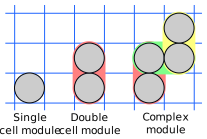
\includegraphics[width=0.7\textwidth]{figures/rofi_shapes.pdf}
    \caption{Example of a module hull construction. Each convex hull of adjacent
    cells is denoted by a coloured area. The module hull is the union of coloured
    areas. Note that the coloured areas slightly overlap the grid. This is only
    for the purpose of visualization. In reality they fit exactly in the grid.}
    \label{fig:rofi_shapes}
\end{figure}

The modules are allowed to change their shape by offering several degrees of
freedom in the form of \emph{joints}. Joint is a single rotational or linear
degree of freedom. Intuitively, we can view a module as beads, which can rotate
against each other along the axes of joints. For a simple example of a double
cell module movement see figure \ref{fig:grid_aware}.

The motivation for such a restriction of the shape is a property we call
\emph{grid-awareness}. Consider a simple task for a double cell module: having a
grounded left part of the module, move its right part above the left one.
Figure~\ref{fig:grid_aware} illustrates the task. If we consider a module which
fits exactly inside a cube-shaped cell, e.g. an M-TRAN module
\cite{haruhisa_kurokawa_m-tran_2003}, the module occupies extra cells during the
movement (marked by red circles in the figure). Such shape restricts the module
movement in a densely occupied grid. However, if we consider a grid-aware module
(e.g., double cell module), it only occupies the minimal number of cells
necessary for the movement and as a result. it should allow for more efficient
reconfiguration algorithms. The key to grid-awareness is the sphere inscribed in
a cell. Therefore, Roombots \cite{bonardi_locomotion_2012} are not grid-aware
even though their shape is a sphere. Their bodies cannot be inscribed in spheres
inside grid cells. Grid-awareness, however, comes at a cost. It requires a
retractable docking mechanism as two neighbouring modules can feature only point
contact. We further discuss this in section \ref{sec:dock} and section
\ref{sec:dock_in_grid}, where we define allowed positions for docks on a module.

\begin{figure}[!t]
    \centering
    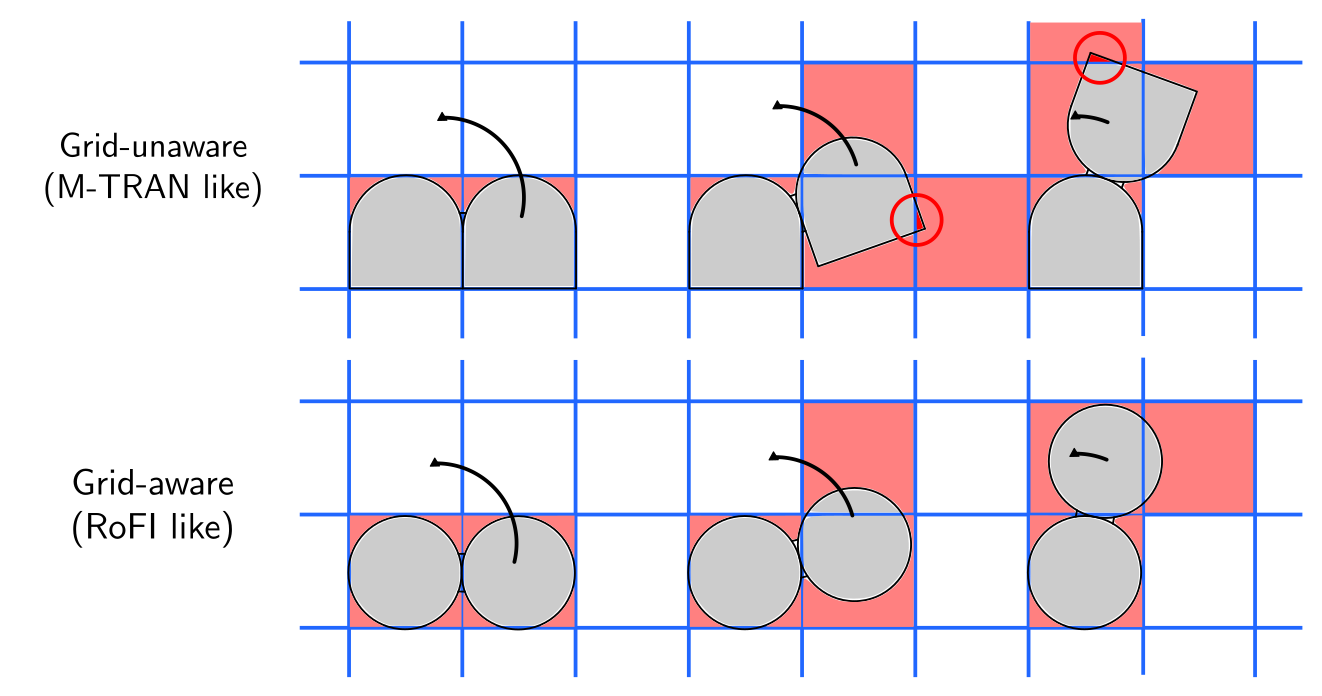
\includegraphics[width=\textwidth]{figures/grid_aware.pdf}
    \caption{Visualization of grid-awareness. Consider two module shapes --
    M-TRAN \cite{haruhisa_kurokawa_m-tran_2003} like (in the top row) and a RoFI
    like (in the bottom row). Given the task to move right body over the left
    one, M-TRAN like module occupies extra cells due to small parts of its body
    overlapping out of the gird. That is not true for the RoFI like module as it
    occupies the least number of cells required to make the movement. }
    \label{fig:grid_aware}
\end{figure}

We want to point out that even though we showed grid-fitting positions of the
robots (where all movement is performed by steps of $90^\circ$) in all examples,
we do not give any restriction on the granularity of the movement. We assume the
modules are physically able to move practically continuously (considering limits
of a mechanic construction). However, the reconfiguration algorithms built on
top of the system can take only discrete steps in the movement into account if
they need to.

The shape specification allows us to define modules with various shapes and
functionality. However, we do not expect the platform to feature many different
types of modules and especially oddly shaped ones. We firmly believe that the
double cell universal module (described in chapter \ref{chap:universal_module}),
should be the primary building block of RoFI systems. However, in future, we
consider having, e.g., a passive module (built only from a mechanical
construction), accumulator module or single-cell modules featuring specialized
sensors (e.g., camera) or actuators (e.g., robotic hand or a wheel).

\section{RoFI Docking System}\label{sec:dock}

Since the modules in the RoFI platform are grid-aware, we cannot adapt existing
docking systems from systems like Roombots \cite{bonardi_locomotion_2012} or
M-TRAN III \cite{kurokawa_distributed_2008}. The reason is that two adjacent
modules in the grid feature only a~single point contact and not a whole face
contact as it is common in other modular robotic platforms. Therefore, there is
a need for a retractable dock (see figure \ref{fig:rofi_locking_example}).

\begin{figure}[t]
    \centering
    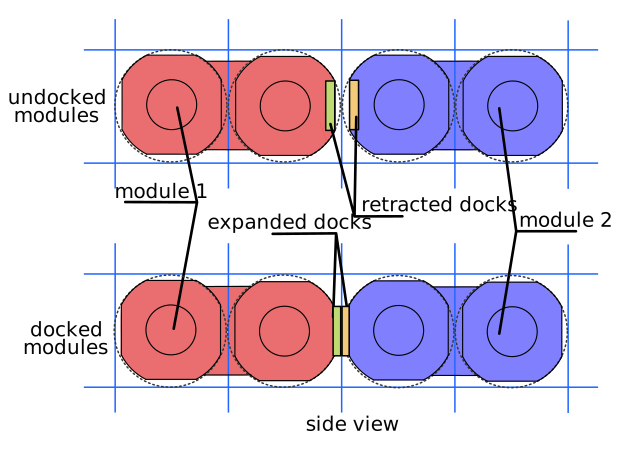
\includegraphics[width=\textwidth]{figures/rofi_locking_example.pdf}
    \caption{Docking procedure. There is a by-default retracted docking system
    in the module which expands when the docking should be performed.}
    \label{fig:rofi_locking_example}
\end{figure}


\begin{figure}[t]
    \centering
    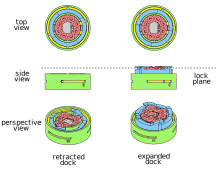
\includegraphics[width=\textwidth]{figures/dock_overview.pdf}
    \caption{The dock from the RoFI docking system. The model is simplified.}
    \label{fig:dock_overview}
\end{figure}

To overcome this issue, we present the RoFI docking system (figure
\ref{fig:dock_overview}). The RoFI system is inspired by the HiGen docking
system \cite{parrott_higen:_2014}. In short, our dock:
\begin{itemize}
    \item allows for connection of two modules when they are not touching side
    by side,
    \item allows for connection in four different orientations,
    \item is genderless (any two docks can connect),
    \item is based on a mechanical connection (and therefore it is not
    limited by a magnetic force and drains energy only during docking and
    undocking),
    \item can disconnect without participation of the mating side (which also
    allows for connecting to a passive dock -- similar to Roombots
    \cite{bonardi_locomotion_2012}) and
    \item supports data communication and power sharing.
\end{itemize}

The docking system is designed to be a stand-alone unit, which can be mass
produced and reused in all modules. It defines a communication interface between
two docks (described in section \ref{sec:dock_interaction}) and communication
interface between a module control unit and the dock (described in
\ref{sec:dock_interface}).

\subsection{The Principle of Operation}

The main principle of operation is the same as the principle of the HiGen dock.
There are two key components -- clip and skirt (figure
\ref{fig:dock_key_components}). The clip features four hooks. These hooks can
slide under hooks of the clip from the mating side and form a connection which
prevents pulling the docks apart. When two skirts touch each other, they stop
the two mating docks from rotating against each other. By combining these two
types of joints, we obtain a firm connection between the two docks.

The operation of a single dock is straightforward -- see figures
\ref{fig:dock_overview} and \ref{fig:dock_description}. Consider a dock in the
retracted position. When the shaft ring (yellow) starts to rotate, it translates
the motion to the clip (blue). There is a helical slot in the dock body (see
figure \ref{fig:dock_key_components}) which forces the clip to move upwards (to
``unscrew''). As the clip moves upwards, it carries the skirt. The skirt moves
in a slot which prevents it from rotating against the body and therefore it only
slides upwards. So far, the clip extends to a locking distance. However, the
hooks of the docks could not slide under each other. A horizontal part ends the
helical slot (see figure \ref{fig:dock_key_components}). This ending allows for
sliding the hooks under each other. The pressure on the hooks and skirts causes
force only in the Z direction; there is no need to hold the components in
position by an active element (e.g., motor) and therefore energy is only
required to change state.

\begin{figure}[t]
    \centering
    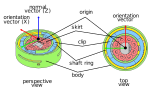
\includegraphics[width=\textwidth]{figures/dock_description.pdf}
    \caption{Naming of the components of the dock. The orientation and the
    normal vector are important for specifying the orientation of two connected
    docks. }
    \label{fig:dock_description}
\end{figure}

\begin{figure}[t]
    \centering
    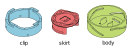
\includegraphics[width=\textwidth]{figures/dock_key_components.pdf}
    \caption{View of the three key components of the dock: a clip, a skirt and
    a body.}
    \label{fig:dock_key_components}
\end{figure}

See figure \ref{fig:dock_locking_process} for an example of an interaction of
two docks. Situation~1 shows the docks in a position such that the connection
plane represents the boundary between two adjacent cells. By rotation of the
shaft ring, the clips and skirts extend (situation 2). Situation 3 shows fully
expanded clips and skirts. The skirts are now connected, and no rotational
movement of the docks is possible. By further rotation of the shaft ring, the
hooks slide under each other and finish the docking process (situation 4).

\begin{figure}[!ht]
    \centering
    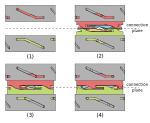
\includegraphics[width=\textwidth]{figures/locking_process.pdf}
    \caption{Illustration of the docking procedure. The clip of the upper dock
    is shown red, the skirt of the upper dock is shown blue, the clip of the
    bottom dock is shown green, the skirt of the bottom dock is shown yellow.
    Situation (1) is the retracted state. The docks pass by the lock plane (2),
    then continue expansion (3) and finish by purely rotational movement (4). }
    \label{fig:dock_locking_process}
\end{figure}

There are two crucial observation to note:
\begin{enumerate*}
    \item the docks are symmetric; therefore there are 4 different orientation
    the docks can lock in;
    \item the movement of two docks does not have to be synchronized, and
    therefore, it is possible for a dock to wait in expanded position or to
    disconnect when the mating module stops responding.
\end{enumerate*}
The absence of the necessity for synchronization can also be leveraged for the
construction of passive docks. Passive dock is a component with no moving parts
in a shape of an extended dock, which an active dock on a module can connect to.

The symmetry of the dock is best shown on the skirt -- see figure
\ref{fig:dock_skirt_symmetry}. There are four identical blocks on the skirt
along the horizontal and vertical axes. The blocks allows for four different
orientation of the docks. When two skirts are facing, there is a mapping of
blocks from one skirt to the other one. The facing blocks have the property that
the green circle is always facing a red one. This feature is vital for
three reasons:
\begin{itemize}
    \item There are pins on the skirt, which prevents the skirt from
    rotation against another skirt (see perspective view in figure
    \ref{fig:dock_key_components}).
    \item Also, there are magnets in the holes (red -- north facing up, green --
    south facing up) which attract the skirts to each other. The magnets help
    misaligned docks to connect correctly.
    \item By mounting spring contacts in the symmetry blocks, we can build power
    and data transmission lines between modules -- see section
    \ref{sec:dock_interaction} for detailed description.
\end{itemize}
The idea behind symmetry of the clip is the same as the idea behind the skirt
symmetry.

\begin{figure}[!ht]
    \centering
    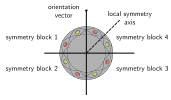
\includegraphics[width=0.8\textwidth]{figures/skirt_symmetry.pdf}
    \caption{Illustration of the skirt symmetry.}
    \label{fig:dock_skirt_symmetry}
\end{figure}

\subsection{Dock Mechanical Implementation}

We designed the dock to be compatible with the 10cm grid. Therefore the dock is
cylindrical, measuring 50~mm in diameter with a depth of 16~mm and can expand up
to 7~mm (module face-to-face distance 14~mm). Compared to the HiGen dock, we
feature half the depth (HiGen depth is 32~mm) while having slightly larger
docking distance (7~mm in our case, 6~mm in the case of HiGen). The thin profile
was achieved by swapping positions of the clip and skirt -- in our case, the
clip is the outer ring and skirt is the inner ring, in the HiGen case skirt is
the outer ring and clip is the internal one. The swap allowed for placing the
motor flat (figure \ref{fig:dock_internal_arrangement}) and therefore, flatter
profile of the dock was achieved. Flat dock profile is a significant advantage
-- the inside of the body can be larger compared to a non-flat profile.

\begin{figure}[!ht]
    \centering
    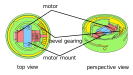
\includegraphics[width=\textwidth]{figures/dock_arrangement.pdf}
    \caption{Internal arrangement of the components inside the dock. Note that
    the skirt and the clip are not shown. The skirt and clip are swapped
    compared to the HiGen dock. This, together with a bevel gearing allow for
    placing the motor flat and therefore, achieving half the depth of the dock.}
    \label{fig:dock_internal_arrangement}
\end{figure}

Note that the depth is independent on the diameter. The diameter choice is a
trade-off between connection stability (increases with diameter) and module size
(also increases with diameter) as we explain in section \ref{sec:dock_in_grid}.
We designed our model to be parametric -- it is possible to specify desired
diameter, connection distance and material thickness, and generate a new model.
The depth of the dock $h$ is equal to $h=l+6w$, where $l$ is the connection
distance (in our model 7~mm) and $w$ is wall thickness (in our model 1.5~mm).
Note that the parameters for the model cannot be chosen arbitrarily as there
some limitations (e.g., in the motor size).

The dock composes of 5 custom components:
\begin{enumerate*}
    \item body,
    \item shaft ring,
    \item clip,
    \item skirt and
    \item motor mount.
\end{enumerate*}
We built several prototypes of the components using a 3D printer. We describe
the process and present the CAD models in chapter \ref{chap:prototypes}. We
believe that with only small modifications, these parts could be lathed and
milled from metal and therefore, being stronger. We build this assumption on
a~similar component complexity as the ModRED docking system
\cite{hossain_towards_2014}. However, even the 3D printed dock provides enough
strength to support small RoFI systems as we show in chapter
\ref{chap:prototypes}.

As we mentioned, the dock is supposed to be a reusable stand-alone unit.
Therefore, there will a PCB with driver electronics in the back of the dock.
However, current prototype does not feature it. The purpose of the electronics
is to:
\begin{enumerate*}
    \item drive the motor in the clip,
    \item buffer incoming communication from an attached dock,
    \item provide a bus interface for a master controller in the module to
    easily control the dock, and
    \item provide an interface for power sharing.
\end{enumerate*}
The electronics is supposed to be rather simple -- small microcontroller is
supposed to drive H-bridge for the motor, detect the limit position of the
mechanism via hall sensors and appropriately placed magnets. Usage of hall
sensors instead of mechanical switches allows for further minimization compared
to the HiGen dock.

\subsection{Mutual Orientation of the Docks}\label{sec:mutual_orientation}

The docks can connect in four different \emph{mutual orientations}. To uniquely
name them\footnote{Naming is used to describe configurations in section
\ref{sec:configuration}.}, we use the \emph{orientation vector} shown in figure
\ref{fig:dock_description}. When two docks connect, there can be an angle of
$0^\circ$, $90^\circ$, $180^\circ$ or $270^\circ$ between their orientation
vectors (measured counterclockwise from a perspective one of the modules;
looking from shoe center to the dock center). Notice that the angle is the same
no matter which module we choose. Therefore, we give a following convention: If
we aim one of the orientation vectors up (to the \emph{north}), the other vector
aims either:
\begin{enumerate*}
    \item \emph{north},
    \item \emph{east},
    \item \emph{south} or
    \item \emph{west}
\end{enumerate*}
as shown in figure \ref{fig:dock_orientation}. Therefore, we define the mutual
orientation $o$ to be an element of $\mathcal{O} = \{N, E, S, W\}$.

\begin{figure}[!ht]
    \centering
    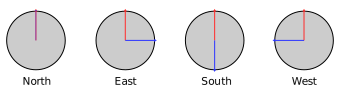
\includegraphics[width=\textwidth]{figures/dock_orientation.pdf}
    \caption{Possible orientation of two docks. The orientation vector of the
    current perspective is shown red, the orientation vector of the mating dock
    is shown blue. Note that it does not matter which dock's perspective we
    choose.}
    \label{fig:dock_orientation}
\end{figure}


\subsection{Docks Interaction}\label{sec:dock_interaction}

When two docks are connected, they can exchange binary blobs and share power.
The communication and power sharing is accomplished by mechanical contact using
pogo pins placed in the inner part of the skirt. The communication between two
docks is implemented as a simple UART (Universal Synchronous Receiver and
Transmitter).

To allow docks to connect in four different mutual orientations and to preserve
the ability to communicate and share power, we use a similar pin arrangement as
the HiGen dock \cite{parrott_higen:_2014} shown in figure \ref{fig:dock_pins}.
The pins are arranged such that in each orientation one of the pin sections A or
B is in contact with one of the pad sections 1 or 2. There are four pins in
total; two pins for power-sharing (GND and 48 V), one pin for UART (TX pin to RX
pad) and a dedicated sense pin for detection of the mutual orientation. The
orientation could be retrieved by detecting which communication line is active,
however, we find such a solution much more complicated. The dedicated sense pin
can also easily recognize if the mating site is still attached.

\begin{figure}[t]
    \centering
    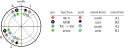
\includegraphics[]{figures/dock_pins.pdf}
    \caption{Pin arrangement on the dock skirt. }
    \label{fig:dock_pins}
\end{figure}

Mutual orientation detection works by permanently pulling the sense pad 1 low
and the sense pad 2 high (over a protection resistor) as shown in figure
\ref{fig:dock_block}. Exactly one of the pins sense A and sense B will be either
pulled low or pulled high; the other one will float. The mutual orientation can
be determined by the table in figure \ref{fig:dock_pins}.

The docks communicate over UART \footnote{The communication speed is easily
achievable due to a short physical communication distance.} with 8 bits, no
parity and a 1.5 stop bit at 6 Mbaud/s. The words are transmitted in
little-endian byte order. The communication protocol between two docks is simple
as the only allowed operation is to pass one binary blob from one dock to
another. The blobs are wrapped in a frame with the following format:

\bigskip
\begin{bytefield}{32}
    \bitheader{0,7,8,15, 16, 31} \\
    \bitbox{8}{\texttt{0xAA}}
    \bitbox{8}{\textit{reserved}}
    \bitbox{16}{content type} \\
    \bitbox{16}{payload length} & \bitbox[r]{16}{} \\
    \wordbox[lbr]{2}{payload} \\
    \bitbox{32}{CRC}
\end{bytefield}
\medskip

\noindent The frame is transmitted to the mating dock over UART. If the mating
dock is unable to handle the incoming frame or the frame is corrupted (CRC
mismatch), the dock can discard the frame\footnote{This behavior mimics the
Ethernet interface and simplifies implementation of the dock.}. Bytes of the
outcoming frame are required to be sent consequently with no additional delay.
There is a silent period of 8 bytes (14 \si{\micro\second}) after each frame.
The receiver should discard incomplete frame after the silent period and prepare
for a next incoming frame. The hardware can implement baud rate correction
algorithms and leverage the constant header 0xAA for this purpose. The content
type field identifies the content in payload and allows to transmit various
protocols over the docks, (e.g., IP datagrams, RoFI debug messages, RoFI
firmware upgrades etc.). The dock is allowed to treat different content
differently (e.g. rearrange them in send buffer, drop them, etc.).

\begin{figure}[t]
    \centering
    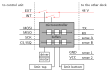
\includegraphics[width=0.9\textwidth]{figures/dock_block.pdf}
    \caption{Block diagram of the dock functionality.}
    \label{fig:dock_block}
\end{figure}

\subsection{Dock Power-sharing}

The connection of two docks is direct with no galvanic isolation. Therefore the
modules in the RoFI systems are required to share the same ground potential or
float before the connection is performed. The power is shared on a single 48~V
line. We choose a 48 V line to mitigate the power losses on the conductors.

The dock exposes two power lines to the module -- \emph{EXT} and \emph{INT}. The
EXT line is required to be directly connected to all EXT lines of the other
docks in a module. The purpose of the EXT line is to share power between
connected devices. The INT line is supposed to power the module and, e.g.,
charge an internal accumulator. The internal wiring diagram (figure
\ref{fig:um_internal} servers as a reference example for connection of the lines
in a module. Both of these lines can be connected to or disconnected from the
source independently. The hardware implementation of the switch is shown in
figure \ref{fig:dock_biswitch}. A simple transistor switch is not enough as the
current can flow both directions. The switch will also monitor the line voltage
and measures the current via electromagnetic coupling.

\begin{figure}[t]
    \centering
    
\includegraphics[width=0.7\textwidth]{figures/dock_biswitch.pdf}
    \caption{Implementation of a bidirectional switch in the dock.}
    \label{fig:dock_biswitch}
\end{figure}

The separation of the power lines into the EXT and INT lines allows for
different modes of operation:
\begin{enumerate}
    \item The module does not participate in power-sharing (all switches are
    opened). The module serves as an isolator and can be used to separate
    the system into several independent power-sharing components.
    \item The module connects the docks to the EXT line. The module servers a
    power bridge, but does not drain nor source any power to the system.
    \item One or more docks are connected to the INT line. The module can drain
    power from or source power to the system.
    \item The previous modes are combined -- e.g., two docks are connected to the
    EXT line and therefore, can share power, but the module is connected to
    another dock.
\end{enumerate}

The RoFI modules are expected not to share power by default. The power sharing
mechanism should not by default connect all the modules in a system. The modules
should run on their own accumulator and only if a module in the module requires
external power, the circuit from the EXT lines should be established and the
energy should be transferred.

\subsection{Dock Interface}\label{sec:dock_interface}

The docks in a module should be controlled by the module control unit. There are
usually multiple docks in a single module.

The dock provides SPI slave interface on 3.3 \si{\volt} level to control the
dock (figure \ref{fig:dock_block}). The chip select pin (CS) also serves as an
interrupt to the master -- when an interrupt is issued, the pin is pulled low by
the slave. Words are transmitted in the little-endian byte order, bytes are sent
most-significant bit first. The data are read at the rising edge of the clock
signal. The dock should support at least 10 \si{\mega\hertz} clock signal.

There can be multiple variants of the docks (e.g., variants featuring sensors).
There is unique number identifier assigned to each dock variant. So far, we
specify only dock variant 1 with no sensors, further referenced as a \emph{base
dock}. The following text describes revision 1 of the communication protocol.
Future revisions might be released, but they must be backward-compatible.

The communication on the bus is performed in transactions -- each transaction
starts by master pulling CS low and end by releasing CS back to high. Incomplete
transactions must have no observable effect. Each transaction follows the format:

\bigskip
\begin{bytefield}{32}
    \bitheader{0,7,8} \\
    \bitbox{8}{command} & \bitbox{24}{command data} \\
    \wordbox[tb]{2}{pause at least 8 bytes (no clock)}  \\
    \wordbox{2}{dock response/extended data}
\end{bytefield}

\noindent Both, command data and the dock response, require no padding. The
commands 0--127 are reserved for the base dock, and all dock types are required
to support them. The commands 128--255 are dock type specific. The basic
commands are:

\paragraph{Version command (0):} has no command data. The response is in the
format:

\bigskip
\begin{bytefield}[bitwidth=1.75em]{16}
    \bitheader{0, 15} \\
    \bitbox{16}{dock variant} \\
    \bitbox{16}{protocol revision}
\end{bytefield}

\paragraph{Status command (1):} can be used to query dock status and issue
status changing commands like expanding or retracting the dock. We consider
following bitfields for this command:
\begin{itemize}
    \item P (position, 1-bit) -- 1: expanded dock, 0: retracted dock,
    \item I (internal, 1-bit) -- 1: the INT line is connected, 0: the line is disconnected,
    \item E (external, 1-bit) -- 1: the EXT line is connected, 0: the line is disconnected,
    \item C (connected, 1-bit) -- 1: the dock is connected (the sense pin is
    active), 0: the dock is disconnected and
    \item O (mutual orientation, 2-bit) -- 0: north, 1: east, 3: south, 4: west.
\end{itemize}

The command data consist of two parts a status bitmask and a write mask. By
setting a corresponding bit in write mask, we can change the state of the
corresponding feature of the dock to the state specified by a status bitmask.
E.g., by setting bit I to 1 and setting corresponding bit in write mask, the INT
line will be connected. Zeroes in the write bitmask are left unchanged. The
format of the command data is:

\bigskip
\begin{bytefield}[bitwidth=1.75em]{16}
    \bitheader{0-15} \\
    \bitbox{1}{P} &
    \bitbox{1}{I} &
    \bitbox{1}{E} &
    \bitbox{13}{\textit{reserved}} \\
    \bitbox{3}{write mask} &
    \bitbox{13}{\textit{reserved}}
\end{bytefield}

\noindent The dock response follows the similar format as the command. The dock
returns the status before performing the command. It also sends the count of
blobs waiting in the buffer for transmission, count of blobs not retrieved by
the master and voltage and current on the power lines. The voltage is in 8.8
fixed-point number in volts, the current is in 8.8 fixed-point number in
Amperes. The format is following:

\bigskip
\begin{bytefield}[bitwidth=1.75em]{16}
    \bitheader{0-15} \\
    \bitbox{1}{P} &
    \bitbox{1}{I} &
    \bitbox{1}{E} &
    \bitbox{5}{\textit{reserved}} &
    \bitbox{1}{C} &
    \bitbox{2}{O}
    \bitbox{5}{\textit{reserved}}\\
    \bitbox{8}{blobs pending to send} & \bitbox{8}{blobs pending to retrieve} \\
    \bitbox{16}{INT line voltage (8.8 fixed-point)} \\
    \bitbox{16}{INT line current (8.8 fixed-point)} \\
    \bitbox{16}{EXT line voltage (8.8 fixed-point)} \\
    \bitbox{16}{EXT line current (8.8 fixed-point)}
\end{bytefield}

\paragraph{Interrupt command (2):} can be used to query interrupt reason and to
enable and disable interrupts. There are following interrupts:

\begin{itemize}
    \item C -- connect or disconnect event occurred (the sense pin change) and
    \item I -- new binary blob received.
\end{itemize}
The data command is a bitmask with enabled interrupts:

\bigskip
\begin{bytefield}[bitwidth=1.75em]{16}
    \bitheader{0-15} \\
    \bitbox{1}{C} &
    \bitbox{1}{I} &
    \bitbox{14}{\textit{reserved}}
\end{bytefield}

\noindent The response follows the same format:

\bigskip
\begin{bytefield}[bitwidth=1.75em]{16}
    \bitheader{0-15} \\
    \bitbox{1}{C} &
    \bitbox{1}{I} &
    \bitbox{14}{\textit{reserved}}
\end{bytefield}

\noindent Bits set to 1 signal interrupt reason. After the response is sent, all
interrupt reasons are cleared. Therefore, the mask returns all interrupts
reasons from the last query.

\paragraph{Send blob (3)} is used to send a binary blob. There are no command
data. The extended data are formatted as follows:

\bigskip
\begin{bytefield}[bitwidth=1.75em]{16}
    \bitheader{0, 15} \\
    \bitbox{16}{content type} \\
    \bitbox{16}{blob length} \\
    \wordbox{2}{blob data}
\end{bytefield}

\noindent The size of a blob should be less than 1500 bytes (to be compatible
with Ethernet). However, the dock might supporter larger blobs.

\paragraph{Receive blob (4)} is used to obtain a received blob from the mating
dock. The oldest received blob is sent. The command has no data. The response
follows the format:

\bigskip
\begin{bytefield}[bitwidth=1.75em]{16}
    \bitheader{0, 15} \\
    \bitbox{16}{content type} \\
    \bitbox{16}{blob length} \\
    \wordbox{2}{blob data}
\end{bytefield}

\noindent If there are no pending blobs, a blob of zero length is returned.

\subsection{Docks in the Grid System}\label{sec:dock_in_grid}

The shape requirements in section \ref{sec:aware} omitted the placement of the
docks. As we have already defined the RoFI dock in this section, we can complete
the shape requirements with possible dock placements.

Consider a shoe, the basic abstract building block of modules (figure
\ref{fig:dock_positions}). We define the origin of the shoe in the middle of the
sphere. There are up to 6 adjacent shoes in the grid (in both direction of all
axes X, Y, and Z.) The directions define six possible dock positions which we
name after an axis direction. We name it $\mathcal{P} = \left\{+X, -X, +Y, -Y,
+Z, -Z\right\}$. We also give an orientation of the dock (see figure
\ref{fig:dock_positions}).

Therefore, each RoFI module can specify a subset of docks it features for each
cell it occupies. Once we introduce module descriptors in section
\ref{sec:capabilities}, we will be able to name each dock unambiguously.

\begin{figure}[t]
    \centering
    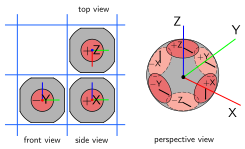
\includegraphics[width=\textwidth]{figures/dock_positions.pdf}
    \caption{There are 6 positions for the docks on a shoe -- in the
    centers of faces of the corresponding cell cube. The docks are named using
    the axes names. Small arrows denote the orientation vector of each dock.}
    \label{fig:dock_positions}
\end{figure}

\section{Inter-module Communication}\label{sec:communication}

Inter-module communication is an essential part of a modular robotic system.
Without it, there is no space for emergent behavior to form. There are two
possible means of communication: wireless one and wired one. Both of them
has its advantages and disadvantages.

The wireless communication is easy to implement, as there is no need to
establish a physical connection between the modules. Absence of physical wiring
simplifies docking mechanism also allows for communication of separate
systems of modules. However, due to its nature, it does not scale well as all
the modules share the same medium and only a single module can transmit at a
time. Also, standard networking technologies like WiFi or Bluetooth are not
suitable for handling possibly hundreds of device in one place, especially in
an embedded environment.

On the other hand, wired communication can scale well as every two connected
modules can communicate without being limited by the other modules. It can also
be more power efficient compared to the wireless one. As there is already a need
for physical connection, a power-sharing interface can be added at minimal cost.
Therefore the connected modules can share and distribute energy. Unlike the
wireless one, there is a need for routing as there is no shared medium and only
adjacent modules can communicate.

The RoFI platform relies primarily on a wired communication between every two
connected modules and optionally allows for wireless communication. This
design choice allows for fast and parallel communication inside a single system
and also allows to establish a communication with a remote system.

With the RoFI platform we do not want to reinvent the wheel and, e.g., come up
with a custom communication and routing protocol based on RS-485 like M-TRAN or
the CAN in case of the HyMod project \cite{parrott_hymod:_2016}. For example,
the CAN bus is fault tolerant and provides prioritized messages, however for
purposes of modular robots, it features several disadvantages:
\begin{enumerate*}
    \item it has a limited bandwidth of 1 Mb/s \cite{noauthor_road_2013},
    \item it does not scale well as all devices share the same medium,
    \item cannot be cyclic and therefore, needs bus switches to remove cycles,
    \item needs an adjustable impedance based on the topology
    \cite{parrott_hymod:_2016}.
\end{enumerate*}

Therefore, the RoFI platform leverages traditional computer network based on the
TCP/IP protocol and stack. The TCP/IP protocol allows for seamless operation
with existing computer networks and services. The users can use traditional
sockets, port OpenMPI to their projects or use the network for sending debug
logs from the distributed environment. It potentially opens doors for global
communication of the RoFI systems. Using TCP/IP also makes indistinguishable
wired and wireless connection from each other. Routing and robustness also come
for free. The downside of the TCP/IP stack is its complexity; however, this is
partially compensated by the existence of ready-to-use implementation even for
embedded platforms (eg., lwIP \cite{noauthor_lwip_nodate}).

There are two possibilities to implement the TCP/IP in the platform: either use
Ethernet to connect the modules (making each module to act either as a hub or
switch) or introduce a custom L1/L2 layer of the OSI/ISO model
\cite{braden_requirements_1989}. Note that introduction of custom L1/L2 layers
is quite common (e.g. \cite{lindgren_ip_2008} or \cite{waitzman_ip_1999}).

We have already defined the communication between two docks in the section
\ref{sec:dock}. The dock connection allows us to pass arbitrary packets of data
between two modules. Considering concrete implementation in lwIP, these two
operations, sending a receiving of a packet (possibly with a custom header), is
all that is necessary to implement a custom device driver. A device driver is a
terminology of lwIP and basically is equivalent of the L2 of ISO/OSI model.

We choose to implement a custom physical layer for the RoFI platform
for several reasons:
\begin{enumerate*}
    \item ethernet switching ICs usually feature only up to 5 interfaces, which
    is not enough for the universal module;
    \item routing a board with such a chip is challenging;
    \item the docks cannot share a bus and many wires are required;
    \item ethernet requires electromagnetic coupling for galvanic isolation,
    which is space consuming and the isolation does not make sense in our setup
    due to the presence of power-sharing.
\end{enumerate*}

The usage of TCP/IP also allows us to easily change our choice later, e.g., if
we find current solution too slow, without affecting existing software. Only a
small portion of robot driver would have to change and also, we can combine
multiple physical layers.


\section{RoFI Capabilities}\label{sec:capabilities}

The section \ref{sec:aware} gives an idea about all possible shapes of the RoFI
modules and also provides examples of use cases for shape other than the
universal module. To allow interaction of different modules and also to build
a formal description of RoFI systems, there is a need to establish a way to
describe various modules and their capabilities. There are two aspects to
consider:
\begin{enumerate}
    \item modules have various shapes and can perform various movements and
    \item modules feature various sensors and special functions.
\end{enumerate}

\emph{RoFI descriptors} cover both of these aspects. Descriptors can be
exchanged by the modules when they connect to build a notion of the system which
is essential for any reconfiguration. We distinguish two types of descriptors:
\begin{enumerate*}
    \item \emph{shape descriptor} ($\mathcal{D}_S$) and
    \item \emph{capability descriptor} ($\mathcal{D}_C$).
\end{enumerate*}

We define the shape descriptor $\mathcal{D}_S$ as a tuple $(S, B, E, t, d)$
where:
\begin{itemize}
    \item $S$ is a finite set of shoes,
    \item $B$ is a finite set of bodies,
    \item $E$ is a finite set of edges, formally $E \subset (S\cup B)^2$ such
    that there are no symmetric edges and self-loops,
    \item $t$ is a function returning a transformation function (joint
    transformation matrix) for given edge, formally: $t:
    E\rightarrow(\mathds{R}\rightarrow\mathds{R}^{4\times4})$,
    \item $d$ is a function giving a set of dock present on each shoe. Formally,
    $d: S\rightarrow 2^\mathcal{P}$.
\end{itemize}
Intuitively, $\mathcal{D}_D$ is an oriented graph, with two types of nodes --
shoes and bodies, where edges are labeled by functions returning 3D
transformation matrices. Note that the graph can be cyclic; however, for each
pair of vertices, there is at most one edge. When drawing descriptors we denote
shoes as circles, bodies as squares and we write the functions on edges. See
an example of such a descriptor for a universal module in figure
\ref{fig:um_descriptor}.

\begin{figure}[t]
    \centering
    
\includegraphics[width=\textwidth]{figures/um_descriptor.pdf}
    \caption{Shape descriptor for a universal module. See figure
    \ref{fig:um_body_parts} and \ref{fig:um_axis} for a visualization of the
    module and its axes. Function $\text{rot}_A(x)$ returns a 3D rotation matrix
    along axis $A$ and $x$ radians, $\text{trans}_A(x)$ returns a 3D translation
    matrix in direction of axis $A$ and distance $x$ units, $\text{sym}$ returns
    a matrix flipping direction of all axes. $G$ denotes the size of the grid.}
    \label{fig:um_descriptor}
\end{figure}

Each edge with a non-constant function represents a joint. Further in the text
we will abuse the notation a little and name the edges, arguments of the
corresponding transformation functions and corresponding joints by the same name
-- usually by a small Greek letter. The type of the object represented by the
name should be obvious from the context. For example, we name the edge
$(\textsf{shoe A}, \textsf{body A})$ as $\alpha$, the same as the corresponding
joint (figure \ref{fig:um_axis}) and the argument of rotation. Also, for
practical reasons we consider all descriptors to have unique naming of shoes and
bodies (easily achieved by prefixing the name by module name); however, in the
examples, we omit the prefix to make them simple.

Given the joint positions, the shape descriptors allow for easy computation of
shoe positions in the space. The path in a descriptor between two shoes defines
a transformation matrix representing relative the position of the two shoes.
However, finding such a path might not always be possible due to an orientation
of the edges. By defining a function flip for labeling reversed edges such that:
\[\text{flip}(\text{f})(t) = (\text{f}(t))^{-1}, \text{ for every } t \text{ in
range of a corresponding joint}\] an orientation of an edge can be reversed.
Once reversed, the edge is labeled by a function returning inverse
transformation compared to the original label. Therefore, there is a path
between every two shoes in a module\footnote{The module must be weakly
connected by definition.}.

It is possible to extend the idea of module descriptors further to find
positions of the docks. A descriptor of a single shoe can be constructed in the
same manner as a descriptor for any other module (figure
\ref{fig:shoe_descriptor}). The transformations for docks are constant
functions. The coordinate system is transformed such that the axes orientation
is the same as in figure \ref{fig:dock_description} -- the Z axis is
perpendicular to the docks, and the X axis is coincident with the orientation
vector. We do not consider the docks to be a part of the shape descriptor as
they are the same for each shoe and therefore for the sake of simplicity, they
can be omitted. However, we find them useful to consider the following
construction.

\begin{figure}[t]
    \centering
    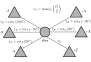
\includegraphics[width=0.8\textwidth]{figures/shoe_descriptor.pdf}
    \caption{Shape descriptor of a shoe. Triangles represent the docks. See
    figure
    \ref{fig:dock_positions} for visualization of a physical layout.}
    \label{fig:shoe_descriptor}
\end{figure}

So far, we considered descriptors only in the context of a single module. We can
further extend it to multiple modules. Two descriptors can be joined by adding
edges between connected docks. The relative position of any two shoes in the
system can be computed using this graph. The construction of the connection is
illustrated in figure \ref{fig:connection_descriptor}. We will refer to this
operation as \emph{shape descriptor union}.

\begin{figure}[t]
    \centering
    
\includegraphics[width=0.8\textwidth]{figures/descriptor_connection.pdf}
    \caption{Illustration of connection of two module descriptors. Each module
    has a shoe (shoe A, shoe B) with docks they connect to each other. To
    connect the modules, a new edge is constructed between the docks.
    Parameter~$o$ is the mutual orientation of the docks. Note that it does not
    depend on the edge orientation as the mutual orientation is symmetric as
    shown in section \ref{sec:mutual_orientation}. }
    \label{fig:connection_descriptor}
\end{figure}

To allow algorithms take various sensors present on modules into an account,
simple sensor enumeration is not enough as the position of the sensor matters.
Therefore, the RoFI platform allows sensors to be placed on faces of the shoe.
The faces are named as the corresponding docks (figure
\ref{fig:dock_positions}). The capability descriptor $\mathcal{D}_C$ is a
function $\mathcal{D}_C: S\times\mathcal{P} \rightarrow 2^{I}$, where $I$ is a
set of all possible sensors. Intuitively, $\mathcal{D}_C$ is a labeling of
individual docks on the module assigning sensors to them. The set of all sensors
$I$ contains sensor-dependent descriptions\footnote{As there exists only the
universal module we consider specification of the sensor format rather
premature.}.

\section{RoFI Configurations} \label{sec:configuration}

So far, we gave means to describe a single module. To ease and unify the
development of a firmware and reconfiguration algorithms, we also give means to
describe a system consisting out of the RoFI modules.

First, there is a globally unique ID (\emph{GUID}) assigned to each instance of
a module. GUID is a 128-bit number to prevent GUID exhaustion. Second, when
talking about RoFI systems, we distinguish two terms:
\begin{enumerate*}
    \item \emph{topology} ($\mathcal{T}$) and
    \item \emph{configuration} ($\mathcal{C}$):
\end{enumerate*}

\paragraph{topology} Intuitively, topology describes the connection between the
modules in a system and does not care about the physical layout of the modules.
Formally, we define a topology $\mathcal{T}$ as a tuple $(M, E, d)$:
\begin{itemize}
    \item M is a finite set of modules represented by GUID, formally $M\subset
    G$, where $G$ is a set of all GUIDs.
    \item E is a finite set of undirected edges (connections) between the
    modules. Note that the undirected edge forces that both modules have to
    actively participate in a connection.
    \item $d$ is a labeling function for edges. The function assigns a set of
    labels to an edge. The labels are tuples in form $(o, d_a, d_b)$, where
    $o\in\mathcal{O}$ is a mutual orientation of connected docks, $d_a$ and
    $d_b$ from modules in the edge. The order of docks in the tuple is given
    lexicographically (first by module GUID, second by the dock name). Therefore
    the labels are canonical.
\end{itemize}

\begin{figure}[t]
    \centering
    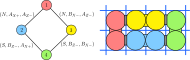
\includegraphics[width=\textwidth]{figures/topology_example.pdf}
    \caption{Example of a topology (left) for a system of the universal modules
    (right). Connections are denoted by gray rectangles, the naming of the docks
    follows figure \ref{fig:um_docks}. }
    \label{fig:topology_example}
\end{figure}

\paragraph{configuration} Intuitively, a configuration is a topology with the
 module joints positions. Formally, a configuration $\mathcal{C}$ is a pair $(T,
 L)$:
 \begin{itemize}
    \item $T$ is a topology and
    \item $L: M \rightarrow \text{A} \rightarrow \mathds{R}$, where $A$ is a
    union of axes from all module types, is a function assigning values to all
    joints in the system.
 \end{itemize}

We define a \emph{model of a topology} $\mathcal{M}_\mathcal{T}$ as a descriptor
obtained by the following procedure:
\begin{enumerate*}
    \item rename uniquely descriptors of each module instance in the system, then
    \item select an arbitrary one and
    \item union the selected descriptor consequently with the other modules
    using module union (defined in section \ref{sec:capabilities}).
\end{enumerate*}
We define a \emph{model} $\mathcal{M}_\mathcal{C}$ of a configuration
$C=(T, L)$ as a model of $T$, where labels were evaluated according to $L$,
i.e., labels are constant values. Configuration $C$ is \emph{realizable} iff:
\begin{enumerate*}
    \item for all pair of shoes, all paths between them in the model of $C$
    yield the same relative position and
    \item no two shoes in the model of $C$ intersect.
\end{enumerate*}

There are no constraints on topology; therefore, we consider every topology
valid. However, for some topologies there exists no realizable configuration.
Given the terminology, there are few aspects to note:
\begin{itemize}
    \item To move the robot means to change a configuration.
    \item Change in configuration can also mean change in topology.
    \item Change in topology always means a change of configuration.
\end{itemize}


\chapter{Universal Module}\label{chap:universal_module}

The chapter \ref{chap:rofi} gives the specification for modules in the RoFI
platform. In this chapter, we present the RoFI \emph{universal module}. This
module is supposed to be the main building block of RoFI systems. It should
provide enough versatility to build vast amount of systems.

This chapter provides overview of the design of the universal module and gives a
specification to implement it. The current state of implementation is discussed
in the chapter \ref{chap:prototypes}.

\section{Universal Module Shape}

The universal RoFI module occupies two adjacent cells of the grid as can be seen
in the figure \ref{fig:um_reference}. Please note that this drawing gives a
simplified model in which many technical details are omitted. The arrangement of
the module is inspired by the M-TRANs \cite{kurokawa_distributed_2008}. Unlike
M-TRANs, the universal module is grid-aware. There are four parts from which the
module is composed:
\begin{enumerate*}
    \item \emph{body A},
    \item \emph{body B},
    \item \emph{shoe A} and
    \item \emph{shoe B}.
\end{enumerate*}
See figure \ref{fig:um_body_parts}. Bodies are supposed to encapsulate
actuators, electronics and accumulators; shoes are meant to provide connection
to other modules and provide movement.

\begin{figure}
    \centering
    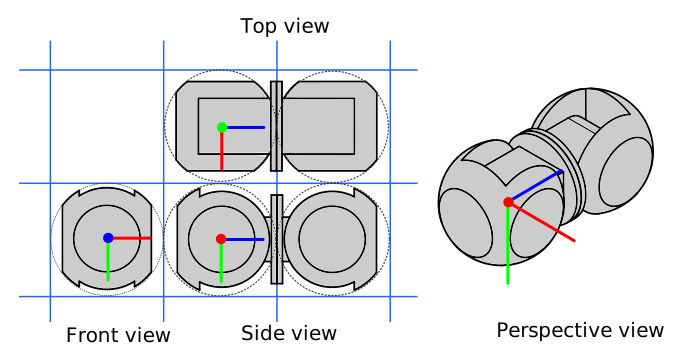
\includegraphics[width=\textwidth]{figures/um_reference.pdf}
    \caption{The universal RoFI module. Blue lines specify the grid, dotted
    lines marks spheres in which the module in inscribed. Note that we show the
    module with the Z axe facing right as it better fits  the page layout. }
    \label{fig:um_reference}
\end{figure}

\begin{figure}
    \centering
    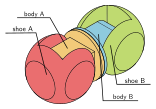
\includegraphics[width=0.7\textwidth]{figures/um_body_parts.pdf}
    \caption{Parts of the universal module.}
    \label{fig:um_body_parts}
\end{figure}

There are 3 degrees of freedom (figure \ref{fig:um_axis}):
\begin{enumerate}
    \item shoe A can rotate against body A along the $\alpha$ axe in a range
    $\langle -90^\circ; +90^\circ\rangle$,
    \item shoe B can rorate against body B along the $\beta$ axe in a range
    $\langle -90^\circ; +90^\circ\rangle$ and
    \item body A can rotate against body B along the $\gamma$ axe in $\langle
    -180^\circ; +180^\circ\rangle$ with an overflow\footnote{First prototypes
    feature a limitation on a number of overflows in one direction the $\gamma$
    axe due to technical limitations. }.
\end{enumerate}
The module should be able to provide at least 1.5 $\text{N}\cdot\text{m}$ of
torque for each axe.

\begin{figure}
    \centering
    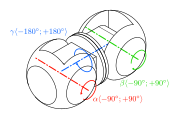
\includegraphics[width=0.7\textwidth]{figures/um_axis.pdf}
    \caption{Degrees of freedom of the universal module. The figure represents neutral position of each joint.}
    \label{fig:um_axis}
\end{figure}

There are 3 docks on each each shoe -- docks $X+, X-$ and $Z-$. The position of
the docks is captured in the figure \ref{fig:um_docks}. Given this setup we
can construct universal module descriptor shown in the figure
\ref{fig:um_descriptor}.

\begin{figure}
    \centering
    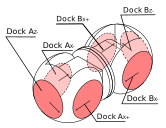
\includegraphics[width=0.7\textwidth]{figures/um_docks.pdf}
    \caption{Docks on the universal module. The arrow on each dock specifies its orientation.}
    \label{fig:um_docks}
\end{figure}

\section{Intramodule Architecture}

\section{The RoFI "BIOS" \todo{Proper naming}}

\section{RoFI lib}

\todo{Something here}
\chapter{RoFI Driver}\label{chap:software}

The RoFI platform does not put any restrictions on the implementation of
modules. However, having all the modules based on the same platform is an
advantage. Therefore, we consider the implementation of the universal module to
be a reference implementation for other modules, and we expect the other modules
to reuse it as much as possible.

Software development for robots and embedded systems is considered to be more
challenging than traditional software development. There are several reasons
why is it so:
\begin{enumerate*}
    \item the microcontroller peripherals have to be mastered,
    \item testing and debugging is harder as the system is not self-contained
    and interacts with the environment, and
    \item the code has to deal with numerous asynchronous events, as tasks have
    to be distributed in time.
\end{enumerate*}

We designed several tools and libraries to tackle these aspects of firmware
development and to make the development more convenient. We call them \emph{RoFI
Driver}. The driver is built on top of the software suite provided for the ESP32
microcontroller, which we sum up in section \ref{sec:hardware}. The driver
provides the following functionality:
\begin{itemize}
    \item it seamlessly integrates the docks into the software environment such
    that TCP/IP networking is available,
    \item the modules can distribute firmware updates automatically, and
    \item there is low-level inter-module logging for debugging purposes.
    \item The driver also provides a high-level interface for controlling the
    motors and sensors. The interface allows for easy handling of asynchronous
    events, and
    \item it is possible to do remote interface calls (i.e., to control another
    module).
\end{itemize}

\section{ESP32 Software Suite} \label{sec:hardware}

We expect the firmware for modules to be developed using standard programming
means for the ESP32 microcontroller. The firmware is developed using C++
facilitated by the ESP-IDF framework \cite{noauthor_esp-idf_nodate}. The
framework provides drivers for microcontroller peripherals. Therefore, the user
does not need to toggle individual bits in peripherals' registers. The framework
also includes FreeRTOS, the standard C and C++ libraries, and offers several
useful libraries (lwIP, Bluetooth library or library for a virtual file
system).

The framework exposes its functionality as a plain C interface. Also, much of
the provided functionality is wrapped in a POSIX-compatible interface. E.g.,
sockets are accessible by both, lwIP interface and POSIX interface. The same
follows for threading; the user can use FreeRTOS API or POSIX interface or can
even leverage C++ STL API.

\section{Networking} \label{sec:networking}

We leverage the lwIP library on the ESP32 to implement networking. To make lwIP
compatible with the docks, we have to provide a new network interface.
All docks in the module appear as a single interface. Therefore, the
implementation performs simple switching to determine the destination dock.

\subsection{Dock Integration}

Technically speaking, we have to provide the following function to lwIP to
implement a new network interface:
\begingroup
\setlength{\rightskip}{0pt plus 1 fil}
\begin{itemize}
    \item \cpp{err_t rofi_if_init(struct netif *netif)}:
    to initialize the \texttt{nettif} structure,
    \item \cpp{err_t rofi_if_output(struct netif *netif, struct pbuf *p,} \\ \cpp{ip_addr_t *ipaddr)}
    to wrap a datagram in custom headers and to transmit the datagram to the
    docks.
\end{itemize}
\endgroup
After a system start, the RoFI driver calls \texttt{netif\_add}. The call
registers a new network interface. After the setup, all the incoming datagrams
are passed to the \texttt{rofi\_netif->input} callback. The callback is set in
the structure by \texttt{netif\_add}. Providing these functions is all what is
needed to integrate docks into the lwIP library.

\subsection{Network Interface Implementation}

The implementation of the network interface is straightforward and somewhat
technical. There are only several aspects worth further comment:
\begin{enumerate*}
    \item mapping IP datagrams to the dock interface,
    \item pairing destination address to docks, and
    \item the relation between switching and routing.
\end{enumerate*}

The docks can pass arbitrary binary blobs marked by the content type specifier
to the mating side. The specifier allows to transmit multiple protocols through
the same interface. In the RoFI driver, there are so far four content type
specifiers: 0 -- IP datagrams, 1 -- an address mapping protocol (defined further
in this section), 2 -- low-level logging (section \ref{sec:logging}), and 3 -- a
firmware update protocol (section \ref{sec:firmware_distribution}).

In order to determine which dock should be used for datagram transmission, a
mapping between destination IP addresses and the outcoming dock is needed. The
mapping is performed by the ARP protocol \cite{plummer_ethernet_1982} in the
ethernet based networks; however, the ARP protocol is not a good choice in the
RoFI environment for the following reasons:
\begin{enumerate*}
    \item the connection between docks is point-to-point and
    \item the ARP protocol relies on MAC addresses of physical interfaces which
    the docks do not provide.
\end{enumerate*}

Therefore, we design a simple \emph{address mapping protocol} instead. The
protocol is used to find IP addresses and GUIDs of the module neighbors. There
are two messages in the protocol: a \emph{mapping call} and a \emph{mapping
response}.

\noindent The \emph{mapping response} follows the format:

\bigskip
\begin{bytefield}[bitwidth=1.75em]{16}
    \bitheader{0,7,8,15} \\
    \bitbox{8}{command (1)} & \bitbox{8}{IP address size} \\
    \bitbox{8}{GUID size} & \bitbox{8}{number of entries ($n$)} \\
    \wordbox{2}{IP address 1} \\
    \wordbox{2}{module GUID 1} \\
    \wordbox{2}{$\vdots$} \\
    \wordbox{2}{IP address $n$} \\
    \wordbox{2}{module GUID $n$} \\
\end{bytefield}

Each module keeps a table with IP addresses and module GUIDs for each dock. The
table can contain multiple entries for each dock even though the docks provide
only point-to-point communication. There are following reasons to do that: it
allows to cluster modules in a system and perform packet switching in the
cluster if the further development finds it suitable (e.g., packet switching has
lower latency), and there can be simple modules in the system not capable of
routing (e.g., an accumulator module). The overhead caused by the extended
packet format is negligible and is worth further extensibility.

On the dock connection, the module actively sends the mapping response message
to the mating side. If there is a change which makes the information sent
previously invalid, a mapping response is sent (e.g., the module has changed its
IP address). Such event-driven approach allows establishing the mapping quickly,
however the module should periodically use the \emph{mapping call} to update
entries in the table to avoid the entries to go out-of-data.

\noindent The \emph{mapping call} follows the format:

\bigskip
\begin{bytefield}[bitwidth=1.75em]{16}
    \bitheader{0,7} \\
    \bitbox{8}{command (0)}
\end{bytefield}

\noindent Note that under normal conditions the table cannot go out-of-date;
this can only happen when a malfunction occurs (e.g., a module resets).

\subsection{Module Address Configuration and Routing}

Each module has to have a unique and valid IP address to communicate in the IP
network. The modules have their unique GUIDs, however, GUID is not a good
candidate for an IP address for several reasons. First, it is longer than IPv4
address, second, it does not follow the standard format of IPv6 address, which
reflects the structure of the network, and therefore, GUID does not allow for
efficient routing. There is no central authority in the network of RoFIs like
there is a router in a traditional network, therefore traditional solutions for
the network address obtaining, like DHCP server, cannot be used. Both, address
configuration and routing in large networks with unstable topology, are still an
area of active research, and there is no standardized solution available yet
(\cite{baccelli_ip_2010} and \cite{ezzouhairi_ip_2005}).

As the RoFI is built on top of the TCP/IP networking, nearly all newly proposed
algorithms for routing (e.g., APM \cite{ezzouhairi_ip_2005}) can be adopted as
their experimental implementation relies on TCP/IP. The same goes for IP address
configuration, e.g., in form of Distributed DHCP server
\cite{nesargi_manetconf:_2002}. However, in the first versions of RoFI driver,
we rely on the basic address autoconfiguration implemented in lwIP and a simple
routing algorithm. These algorithms work fine in small networks. In the future,
we plan to adopt the Distributed DHCP server and the APM routing algorithm.

\section{Low-Level Logging} \label{sec:logging}

When firmware for a microcontroller is developed, programmers usually use a
simple communication interface, typically UART, to print debugging messages.
Using print-based debugging is useful, since a debugger cannot pause most
systems as it is impossible to pause the surrounding environment. UART is
usually used as it is stateless, has nearly no code dependencies and is easy to
set up.

The same approach can be used to debug a single unit, however, collecting data
from multiple UARTs on multiple modules is rather impractical. TCP/IP sockets
can be used instead of UART, however, since they rely on networking in case of
routing malfunction or a system crash, a debug message cannot be delivered.
Therefore, we introduce \emph{low-level logging} in the RoFI driver -- a simple
and robust protocol for sending messages in the RoFI system.

The low-level logging is implemented directly on top of the dock interface and
does not rely on TCP/IP networking. The goal is to emit a string and propagate
it to all modules or a special debugging adapter in the form of a dock, where it
can be transmitted to the programmer. The protocol should be used only for
debugging purposes and should be disabled in release builds as it is built on a
naive flooding algorithm.

The low level debugging uses content type specifier 2 (section
\ref{sec:dock_interface}). There is only one type of message:

\bigskip
\begin{bytefield}[bitwidth=1.75em]{16}
    \bitheader{0,15} \\
    \bitbox{16}{random salt} \\
    \wordbox{2}{message string}
\end{bytefield}

\noindent The string can have a length up to 65519 bytes. There is a set of
message hashes in each module. The set keeps hashes of all received messages.
When a module receives a message, it calculates its hash. If the hash is not
present in the set, it is inserted, and the message is resent to all other docks
in the module. The hashes in the set expire after a given period and afterwards,
the expired hashes are removed from the set. This algorithm ensures all emitted
messages are spread into the whole system. Also, the random salt is necessary to
allow for sending the same messages. Note, that if the expiration period is too
short, it is possible to create a message going through the system indefinitely.
However, for the debugging purposes, we do not perceive it as a limitation.

\section{Automatic Firmware Distribution} \label{sec:firmware_distribution}

It is highly desirable that all modules of the same type run the same firmware
version. If the modules can synchronize firmware automatically, the development
process can speed up. The firmware distribution can be achieved in two ways --
either there is a central authority publishing the firmware, or the modules
check the firmware of their neighbors and update the firmware from them.

ESP32 is a suitable microcontroller for remote firmware upgrades. Traditional
microcontrollers can update their firmware only using a bootloader, a small
program residing in reserved area of flash memory, which is executed after
microcontroller boot. If there is a need for custom update protocol, the custom
bootloader has to be written. However, bootloaders have to be self-contained and
have a restricted binary size. Therefore, sophisticated update protocols are
hard to implement. This is not the case for ESP32
\cite{noauthor_esp-idf_nodate}. The flash memory of ESP32 can be divided into
partitions (e.g., a firmware or a virtual file system partition). In the default
configuration, there are two partitions for firmware. These partitions are used
to implement \emph{over-the-air updates} (OTA). One partition is marked as an
active, and upon boot, the bootloader loads user firmware from the active
partition. Then, during regular operation of the microcontroller, firmware can
be written in the second, inactive, partition. Once the firmware is written and
validated, the active flag of the partitions is swapped. When the
microcontroller reboots, the new firmware is used. OTA updates allow using an
existing codebase in the firmware to perform firmware updates. Therefore
complicated protocols, like an update from an HTTP server can be implemented.

ESP-IDF provides an implementation of OTA update from HTTP server and an
interface for implementing custom updates. The update from HTTP server works by
specifying URL and then the microcontroller periodically polls for new firmware
version. The interface consists of three functions -- one for starting the
update, one for processing a binary blob with a piece of firmware, and one for
committing the changes.

The HTTP server update is an example of a central update. We find it unsuitable
for the RoFI systems for following reasons:
\begin{enumerate*}
    \item each module downloads the firmware separately and therefore the
    protocol does not scale well, and
    \item it relies on working TCP/IP connection and routing. If a firmware
    update breaks routing, the firmware update stops working.
\end{enumerate*}
Therefore, we introduce a decentralized \emph{firmware update protocol} relying
only on a dock connection. By flashing a single module, its firmware distributes
among the other modules in a system. We do not restrict the flashing procedure
-- it can be either flashed by a cable from a PC, or the module can download its
firmware from a central authority (therefore, a hybrid approach can be
achieved).

The protocol works as follows. Each firmware has two symbols built in in the
binary: \texttt{ROFI\_FW\_TYPE} and \texttt{ROFI\_FW\_TIMESTAMP}. The user
specifies the firmware type, the timestamp is automatically added during a
build. Firmware type is a 16-bit unsigned integer, the timestamp is a 64-bit
unsigned integer. There are no restrictions on the meaning of the numbers; it is
recommended that the timestamp are milliseconds since UNIX time epoch. A module
updates only to the same firmware type as it already is and to a newer
timestamp. The firmware type allows the system to consist of various types of
modules.

The firmware update protocol uses content type specifier 3 (section
\ref{sec:dock_interface}). There are four types of messages:

\paragraph{Firmware request} is sent by a module to find out a firmware version
of its neighbors. The answer is the firmware announcement. The message has the
following format:

\bigskip
\begin{bytefield}{32}
    \bitheader{0, 7} \\
    \bitbox{8}{command (0)}
\end{bytefield}

\paragraph{Firmware announcement} is broadcasted by a module to its direct
neighbors when it knows the new firmware. The firmware might not be completely
known to the module, and therefore, there is a field of the known size in the
message. If more of the firmware code is known, a new message is broadcasted.
The message has the following format:

\bigskip
\begin{bytefield}{32}
    \bitheader{0, 7, 8, 15, 16, 31} \\
    \bitbox{8}{command (1)} & \bitbox{8}{\textit{reserved}} & \bitbox{16}{firmware type} \\
    \wordbox{2}{firmware timestamp} \\
    \bitbox{32}{firmware size} \\
    \bitbox{32}{known size}
\end{bytefield}

\paragraph{Firmware chunk request} is sent by a module to obtain a new chunk of
the firmware. It is usually a response to firmware announcement. The chunks are
1024 bytes in length (except the last one), and the allowed offsets are also in
multiples of 1024. The message has the following format:

\bigskip
\begin{bytefield}{32}
    \bitheader{0, 7, 8, 15, 16, 31} \\
    \bitbox{8}{command (2)} & \bitbox{8}{\textit{reserved}} & \bitbox{16}{firmware type} \\
    \wordbox{2}{firmware timestamp} \\
    \bitbox{32}{chunk offset}
\end{bytefield}

\paragraph{Firmware chunk response} is a response to a firmware chunk request.
The message has the following format:

\bigskip
\begin{bytefield}{32}
    \bitheader{0, 7, 8, 15, 16, 31} \\
    \bitbox{8}{command (3)} & \bitbox{8}{\textit{reserved}} & \bitbox{16}{firmware type} \\
    \wordbox{2}{firmware timestamp} \\
    \bitbox{32}{chunk offset} \\
    \bitbox{32}{chunk length} \\
    \wordbox{2}{chunk data}
\end{bytefield}

\noindent First, we illustrate the protocol operation in a system composed of a
single module type. Then, we extend it to arbitrary RoFI systems.

When a first module receives a new firmware, it broadcasts the firmware
announcement. Each module keeps a record of the source of newest firmware
available. It can be either the module itself or one of its neighbors. The
firmware sources are ordered by the timestamp and the known size, and for now,
we ignore firmware types. If a module receives a firmware announcement, it
checks if it is newer than any source known so far. If not, the message is
ignored. Otherwise, it updates the firmware source. When a firmware source
contains a newer firmware than the firmware the module currently runs, it starts
the upgrade procedure. It uses a firmware chunk request to ask the firmware
source for a new firmware chunk. If a newer source of firmware appears, the
current firmware update is aborted and a new update is started. During the
update, the module itself broadcasts a firmware announcement message as new
chunks of firmware are received. In this fashion, the new firmware spreads like
a wave in the system. Note that messages can get lost in the system as docks are
allowed to drop datagrams. Therefore, if the message response times out, the
module broadcasts a firmware request to find a new firmware source.

To support multiple firmware types, the module keeps track of the newest
firmware available for each type. If a firmware announcement updates another
type of firmware than the module type is, it broadcasts the announcement to all
neighbors. If a firmware chunk request for other firmware is received, it is
redirected to the source of that type of firmware and the module remembers the
request. When a response in the form of a firmware chunk is received, the module
redirects the message to the author of the request.

\section{Reactive Blocks Library} \label{sec:rbl}

There are currently two classical approaches to tackle the burden of handling
asynchronous events in languages like C or C++. First, a real-time operating
system (RTOS) can be used with several tasks. Each task handles events in a
synchronous blocking manner. This approach leads to a readable code as the
logic for processing events is kept close together and follows the chronological
flow of the events. However, it might not preserve the lowest possible latency
due to RTOS task switching and also does not scale well as the number of tasks
is usually limited. The second approach uses callback functions which are called
to handle an event. This approach scales well; however, it leads to a
hard-to-read code as the callbacks do not preserve context and are spread all
over the source code. This phenomenon is usually referred to as ``callback
hell''. Also, the code complexity increases tremendously when error handling is
added.

We designed a new solution for handling asynchronous events for the RoFI
platform. We call it \emph{reactive blocks}. The idea behind reactive blocks is
simple -- we use the same principle as callbacks; however, we provide a
syntactical sugar to write them in a chain-like structure to preserve the
chronological flow of event handling. Reactive blocks are inspired by the
ReactiveX library \cite{noauthor_reactivex_nodate} and the ranges-v3 library
\cite{noauthor_range-v3_nodate}.

The reactive blocks will be implemented as a stand-alone RoFI independent C++
library -- \emph{Reactive Blocks Library} (RBL). The library targets all
platforms with C++17 and STL support. The target platforms include standard
variants of x64, ARM and also embedded platforms like ESP32 or ARM Cortex-M. As
the library implementation is a subject of another thesis, we provide only a
brief description of its core functionality and omit some semantical nuances and
the implementation details.

Consider the following (somewhat artificial) scenario: when a noisy distance
sensor overcomes a given threshold (generates an edge), the robot notifies
several other robots (judges) over a network. The judges vote and if a majority
votes yes, the robot flashes a LED. For simplicity, consider a line-based text
communication protocol between the robots and numerous reasonably named
functions.

Standard implementation using a blocking interface might look like this:
\begin{minted}{cpp}
while ( true ) {
    // Wait rising edge debounced by 10 samples
    ring_buffer< int > samples( 10, 0 );
    while ( !all( samples,
                  []( int x ){ return x > threshold; } ) )
    {
        samples.push( sensor.read() );
        delay( 10_ms );
    }
    int sensorValue = average( samples );

    // Perform voting
    std::vector< bool > votes;
    for ( auto& judge : judges ) {
        judge.send( "value: " + std::to_string( sensorValue ) )
        vote = judge.receiveLine() == "yes";
        votes.push_back( vote );
    }

    // Flash an LED
    if ( majority( votes, []( bool vote ){ return vote; } ) ) {
        led.on();
        delay( 200_ms );
        led.off();
    }
}
\end{minted}

The sample code is straightforward and easily readable. By putting the code in a
separate task, we can handle multiple asynchronous events simultaneously.
However, the code does not utilize the whole potential of the underlying
hardware as the network communication is synchronous.

Each asynchronous function traditionally takes a callback function as its
argument. The callback is called, when the operation is finished. The result
value or an error is passed to the callback. The task from our example scenario
could be implemented like this using an asynchronous interface:

\begin{minted}{cpp}
std::vector< bool > votes;
template < typename Callback >
void onJudgeResponse( const std::string& resp, Callback c ) {
    votes.push_back( resp == "yes" );
    if ( votes.size() == judges.size() &&
         majority( votes, []( bool vote ){ return vote; } ) )
    {
        c();
    }
}

template < typename Callback >
void vote( int value, Callback c ) {
    for ( auto& judge : judges ) {
        judge.send( "value: " + std::to_string( sensorValue ), [=] {
            judge.receiveLine( [=]( const std::string& s ) {
                onJudgeResponse( resp, s, c );
            } );
        } );
    }
}

ring_buffer< int > samples( 10, 0 );
timer.every( 10_ms, [&ring_buffer]() {
    samples.push( sensor.read() );
    if ( all( samples,
        []( int x ){ return x > threshold; } ) )
    {
        vote( average( samples ), judges, []{
            led.on();
            timer.after( 200_ms, []{
                led.off();
            });
        });
    }
});
\end{minted}

The code is now fully asynchronous but is hard to read -- it does not preserve
the chronological order of event handling, the user has to think about shared
states and has a lot of nested sections. The need for a shared state arises from
the absence of information in the control flow of the program. E.g., the
function \texttt{onJudgeResponse} has to check if it is the last call of the
function. In the first example, there is no such need as the control captures
the information -- once the if-clause is reached, it is clear all judges voted.

The solution we provide is shown in code snippet below. We do not expect the
reader to immediately understand all details of the code as an explanation
follows. We advise the reader to return to this example during the rest of
this section.

\begin{minted}{cpp}
auto overThreshold( std::pair< int, int > value ) {
    return value.first > threshold;
}

auto is( const std::string& what ) {
    return [=]( const std::string& s ) { return s == what; }
}

auto setLed( bool value ) {
    return [=]() { led.set( value ) };
}

auto sensorStream = timer.every( 20_ms ) >> sensor.read;
auto sensorAverage = sensorStream >> slidingAverage( 10 );
zip( sensorStream, sensorAverage)
    >> debounceOn( overThreshold )
    >> std::get< 1 >
    >> [&]( int sensorValue ) {
        return interleave( judges, [=]( auto& judge ) {
            std::string msg =
                "value: " + std::to_string( sensorValue );
            return judge.send( message )
                    >> judge.receiveLine >> is( "yes" );
        } ) >> majority;
    }
    >> setLed( true ) >> wait( 200_ms ) >> setLed( false );
\end{minted}

The reactive blocks follow a similar idea as the range-v3 library -- we describe
a pipeline for data transformation, however, unlike ranges-v3, the data might be
scattered over time. By describing the pipeline, the user can preserve
chronological ordering of the event handling in the code but also preserves
asynchronicity at the same time. In the traditional future concept, which also
allows for describing a pipeline, the pipeline is only linear and allows only a
single value to pass. The reactive blocks allow for non-linear pipelines and
also allows multiple values to pass through it. Visualization of the pipeline
for the example above is shown in figure \ref{fig:rbl_example_1}.

\begin{figure}[!t]
    \centering
    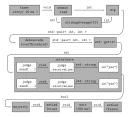
\includegraphics[]{figures/rbl_pipeline_1.pdf}
    \caption{Pipeline visualization for a sensor and a voting code snippet.}
    \label{fig:rbl_example_1}
\end{figure}

Reactive blocks allow chaining data transformation operations -- just like the
UNIX pipe operator. A block represents an operation. There are two types of
blocks: \mintinline[breaklines]{cpp}{template < typename T > Puslisher< T > }
and \mintinline[breaklines]{cpp}{template < typename T > Subscriber< T > }.
A single block can be both publisher and subscriber.

\noindent The publisher can:
\begin{enumerate}
    \item emit an arbitrary number of values of type \texttt{T} at any time (we
    say it generates a \emph{stream} of values),
    \item emit an error (object inheriting from
    \mintinline[breaklines]{cpp}{std::exception}), and
    \item close itself (mark the end of its stream). After closing no more
    values nor errors can be emitted.
\end{enumerate}

\noindent The subscriber can subscribe to a publisher. After subscribing it
\begin{enumerate}
    \item receives values of type \texttt{T} emitted by the publisher and
    \item can unsubscribe.
\end{enumerate}

The interface of a subscriber and a publisher is provided in the
following snipped:
\begin{minted}{cpp}
template < typename T >
class Publisher {
public:
    void subscribe( Subscriber< T >* s );
    void unsubscribe( Subscriber< T >* s );
protected:
    void publish( T t );
    void publishError( const std::exception& e );
    void close();
};

template < typename T >
class Subscriber {
protected:
    virtual void onValue( T t ) = 0;
    virtual void onError( const std::exception& e ) = 0;
    virtual void onClose() = 0;
};
\end{minted}

With these base classes we can derive any other reactive block. For example, we
can build a block which converts a number to a string:
\begin{minted}{cpp}
class N2S: public Publisher< std::string >,
    public Subscriber< int >
{
    virtual void onValue( int i ) override {
        publish( std::to_string( i ) );
    }
    virtual void onError( const std::exception& e ) override {
        publishError( e );
    }
    virtual void onClose() override {
        close();
    }
};
\end{minted}

Or, given a classical callback-based asynchronous interface in the form of a
function \mintinline[breaklines]{cpp}{errorCode asyncFoo( int param, Callback c
)} we can wrap it inside a block which accepts the input for the asynchronous
function and produces an output.
\begin{minted}{cpp}
class AsyncFoo: public Publisher< int >,
    public Subscriber< int >
{
    virtual void onValue( int i ) override {
        errorCode = asyncFoo( i, [&]( int retval ) {
            this->publish( retval );
        } );
        if ( errorCode == ERROR )
            publishError(
                std::runtime_exception( "Something wrong" ) );
    }
    virtual void onError( const std::exception& e ) override {
        publishError( e );
    }
    virtual void onClose() override {
        close();
    }
};
\end{minted}

Similarly, all asynchronous events can be wrapped inside a reactive block --
including interrupts or possibly, but not preferably, busy waiting. Note that
the reactive blocks do not bring asynchronicity to the system, they only
provide a new interface for it. The blocks can also wrap synchronous tasks as
shown in the example of the \texttt{N2S} class. The only requirement is that the
code inside a block should not block for a long time as it might delay other
pending blocks. Also, there can be $m$-to-$n$ mapping of incoming values to the
block, not just 1:1 mapping as we showed in the examples. The block can emit
multiple values from a single input value (e.g., a block splitting string
according to a delimiter or a timer producing values at a given period).

When multiple blocks are linked together via the subscribe relation, we call the
final structure a chain. Therefore, we will refer to the operation as
\emph{block chaining}. Chains are first-class citizens just like blocks.
Therefore we can store them in a variable or chain multiple chains together.

However, building the block manually by defining classes is verbose and leads to
hard-to-read code. Therefore, the library provides an operator
\mintinline[breaklines]{cpp}{>>} (chain). The operator is similar to Haskell's
bind operator -- it builds the subscribe relation between chains. The operator
comes in many overloads and provides an implicit creation of blocks out of
functions. This functionality provides a syntactical sugar, which allows to make
the code less verbose and also allows to keep the code in a chronological order.

To further simplify the code, the library should provide predefined blocks like
zip (takes two streams of values and combines them in pairs), interleave which
takes multiple streams and joins them together, simple waiting, and so forth.

The last advantage of reactive blocks we present is error handling. The
publishers can publish a value or an error. By default, the error goes through the
pipeline until some block stops it and handles it. This provides a monadic- and
exception-like behavior. See the following example:
\begin{minted}{cpp}
a >> b >> c >> onError( []( std::exception& e ) {
    std::cerr "Error a-c: " << e.what() << std::endl();
} ) >> d >> e >> onError( []( std::exception& e ) {
    std::cerr "Error d-e: " << e.what() << std::endl();
} );
\end{minted}
The code defines a linear chain of blocks \texttt{a} to \texttt{e}. If any of
the block fails, the error is captured by one of the two error handlers. Also,
the chain operator by default captures an exception thrown out of functions and
sends them down the chain:
\begin{minted}{cpp}
a >> [] {
    throw std::runtime_error( "Inevidable error" );
} >> b >> onError( []( std::exception& e ) {
    std::cerr "Inevidable error follows:  "
        << e.what() << std::endl();
} );
\end{minted}

In the text above, we presented the library using a runtime polymorphism, which
might not be suitable for embedded platforms. However, for chains with a type
known in the compile time, the runtime polymorphism could be eliminated in the
future releases of the library. The runtime polymorphism elimination also allows
for further optimization and reducing the cost of the reactive blocks
abstraction.

\section{RoFI Driver Interface}

The RoFI interface is provided through a proxy object. The proxy object allows
the user to access various control objects (motors, docks, sensors, \ldots)

The control objects are facades, therefore, they can be copied, which makes
passing them to functions much more convenient. The control objects rely on the
RBL library to implement asynchronous events. E.g., when a joint is commanded to
a position, it returns a publisher; docks provide method \cpp{onConnect()} which
also returns a publisher which emits a value when the dock connects.
Implementing the interface as a proxy brings the possibility to seamlessly
provide remote interface (one module directly controls the other). Such proxy
is an advantage for a centrally controlled system as there is no difference
between controlling itself and any other module.

The reference for the proxy object and control objects can be found in appendix
\ref{chap:rofi_interface}.
\chapter{The RoFI Prototypes}\label{chap:prototypes}

The RoFI project as defined in the previous chapter is broad and, therefore,
implementing all of the proposed solutions in the full depth is far beyond the
reach of the thesis. Therefore, we focused on three of the most important
aspects of the RoFI project. We want to show that:
\begin{itemize}
    \item the docking mechanism can be built and that it features claimed
    properties,
    \item integration of TCP/IP communication in the system using a custom
    hardware layer is possible, and
    \item the universal module can be built.
\end{itemize}

All the source codes and CAD models of results presented here are available at
\url{https://github.com/paradise-fi/RoFi}.

\section{Docking Mechanism}

To test the properties of the docking mechanism proposed in section
\ref{sec:dock} we successfully built several copies of the mechanism and tested
its properties.

The docks can be easily printed on a commonly available 3D printer. In our
setting, the dock was printed on Prusa i3 MK3 using the PLA filament and
standard settings with a layer height of 0.15~mm. We prepared the model for
printing by splitting some complex components into several bodies, which
were printed separately, and after the print they were glued together using
cyanoacrylate glue. As our experiences show, such procedure yields better and
faster results as our model does not need any support material, which needs to
been manually removed. Removing the support material is time-consuming and in
our observation, gluing components together is much faster. Also, surfaces
relying on a support material always yields much worse surface finish than
surfaces with no supports. This is crucial for our model, as a bad surface
finish on the helix slot negatively affects the dock.

Overall, to build a single dock following material is needed: eight meters of a
filament, four M2$\times$6~mm screws with countersunk head, two 2$\times$16~mm
steel pins, four 2$\times$10~mm, four 2$\times$8~mm stell pins and a motor.
Single dock takes about 4 hours to print and with a little bit of practice, it
can be assembled in 30 minutes. Due to tweaks in the design, there is
practically no manual deburring necessary, which is usually required with 3D
printed parts.

We tried to evaluate the features of the dock. However, please note that the
results we present are not as thorough as could be as we do not feature the
equipment and skills to evaluate the mechanical properties of the docks
properly.

\begin{figure}[!t]
    \centering
    \includegraphics[width=\textwidth]{figures/dock_test_setup.jpg}
    \caption{The test setup. A stand was mounted on the docks to easily position
    them and a printed grid was used to create various setups.}
    \label{fig:dock_test_setup}
\end{figure}

\begin{figure}[!t]
    \centering
    \begin{subfigure}[b]{0.45\textwidth}
        \includegraphics[width=\textwidth]{figures/docks_aligned.jpg}
        \caption{Perfect alignment}
        \label{fig:dock_test_aligned}
    \end{subfigure}
    ~
    \begin{subfigure}[b]{0.45\textwidth}
        \includegraphics[width=\textwidth]{figures/docks_distance.jpg}
        \caption{Distance misplacement}
        \label{fig:dock_test_distance}
    \end{subfigure}

    \begin{subfigure}[b]{0.45\textwidth}
        \includegraphics[width=\textwidth]{figures/docks_shift.jpg}
        \caption{Parallel misplacement}
        \label{fig:dock_test_parallel}
    \end{subfigure}
    ~
    \begin{subfigure}[b]{0.45\textwidth}
        \includegraphics[width=\textwidth]{figures/docks_rot.jpg}
        \caption{Rotational alignment}
        \label{fig:dock_test_rot}
    \end{subfigure}

    \caption{Types of displacement.}
    \label{fig:dock_diplacement}
\end{figure}

To properly evaluate the docks, we 3D printed a stand on which a single dock was
mounted. The docks we used for testing were manually controlled. A photo of our
setup can be found in figure \ref{fig:dock_test_setup}. This setup was used for
testing of connection repeatability and load capacity.

\subsection{Connection repeatability}

Two docking mechanisms were brought together in various arrangements and a
series of 10 connects was performed. The docks were placed on a grid to arrange
them in the initial position with one dock being strongly fixed in its position,
the other one being able to move.

First, we performed an analysis of perfectly aligned docks (see figure
\ref{fig:dock_test_aligned}). The connection was established in all 10 cases for
both, simultaneous and sequential docking procedure.

Second, we varied the docking distance (see figure
\ref{fig:dock_test_distance}). By decreasing the docking distance by 6~mm, the
docks were able to push themselves apart and connect properly in all 10 cases.
When the docks were brought together by more than 6~mm, we observed that the
docks are not able to connect simultaneously -- their hooks collide and they do
not align properly. However, when the connection was performed sequentially, the
docks connected reliably event when they were touching as the rotated hooks no
longer collide. By increasing the distance by 2~mm, docks were able to connect
in 9 out of 10 cases. When we increased the distance by 4~mm docks were able to
connect in 5 cases. For displacement larger than 5~mm the docs were not able to
connect.

Third, we varied the parallel alignment (see figure
\ref{fig:dock_test_parallel}). By misaligning the docks by 2~mm we got 9
successfully connections. By increasing the misalignment to 4~mm the docks
connected in 6 cases, for the 6~mm it was only 3 cases. We did not observed ony
difference between simultaneous and sequential attempts.

Last, we varied the rotation of the docks (see figure \ref{fig:dock_test_rot}).
We performed an only rotation in a horizontal plane as the docs are symmetric
and therefore, they should perform the same for other orientations. By rotating
the docks less than $5^\circ$ the docks connected in all 10 cases. When we
increased the rotation to $10^\circ$, we got 7 successful connections for
sequential connection and 5 for the simultaneous connection. For displacement of
$15^\circ$ we got only 1 connection of 10 tries for the sequential connection
and no success for the simultaneous procedure.

When the connection was not successful it was mainly due to the hooks colliding
into each other. The collision usually caused a motor stall, which can be easily
detected by increasing current flow into the motor. This fact could be used by the
robots to detect such collision, and the robots could retry the connection.

\subsection{Load capacity}

\begin{figure}[t!]
    \centering
    \begin{subfigure}[b]{0.45\textwidth}
        \includegraphics[width=\textwidth]{figures/dock_tang_load.jpg}
        \caption{Tangential stress}
        \label{fig:dock_test_tang}
    \end{subfigure}
    ~
    \begin{subfigure}[b]{0.45\textwidth}
        \includegraphics[width=\textwidth]{figures/dock_norm_load.jpg}
        \caption{Normal stress}
        \label{fig:dock_test_norm}
    \end{subfigure}
    \caption{Testing load capacity of the docks. The load was attached to the
    green carabiner.}
    \label{fig:dock_test_load}
\end{figure}

We tested load capacity in two different setups -- in a tangential and a normal
direction (see figure \ref{fig:dock_test_load}) -- by attaching weights to a
carabiner hooked to one of the connected docks. The mating dock was fixed to a
support.

In a normal direction, we were able to repeatably attach a weight of 4.5~kg
until the docks disconnected. The disconnection left no harm on the docks. We
assume the plastic hooks bent under the load as the plastic is quite flexible,
the skirts got loose and therefore, the the docks were able to slip from the
connection.

\begin{figure}[t!]
    \centering
    \begin{subfigure}[b]{0.45\textwidth}
        \includegraphics[width=\textwidth]{figures/dock_damage_1.jpg}
        \caption{Dock hooks}
    \end{subfigure}
    ~
    \begin{subfigure}[b]{0.45\textwidth}
        \includegraphics[width=\textwidth]{figures/dock_damage_2.jpg}
        \caption{Pieces of the hooks broken apart}
    \end{subfigure}
    \caption{Damage caused by load testing on the docks.}
    \label{fig:dock_damage}
\end{figure}

In a tangential direction, we were able to attach weight of 8~kg until the
malfunction of connection happened. In this case, the connection mechanism was
damaged -- two hooks on one dock and one hook on the other dock broke. For a
photo of the damage see figure \ref{fig:dock_damage}. The pieces were broken
between two layers of the 3D printed component. The form of the damage leads us
to a suggestion for future experiments -- printing the hooks such that the
layers of a 3D print are oriented differently.


\section{Inter-module Communication}

We proposed in section \ref{sec:communication} that the modules in a RoFI system
should communicate using a TCP/IP networking as it allows to easily adapt
existing algorithms and technical solutions. The proposed solution implements a
custom layer two of the standard ISO/OSI model.

To show the feasibility of the proposed solution, we have implemented a simple
prototype. The prototype does not provide any mechanical hardware, it consists
only of several interconnected development modules with microcontrollers. We
implemented a firmware for the ATMega328p microcontroller providing the dock
protocol (section \ref{sec:dock_interface}) and a corresponding part of the RoFI
driver for the ESP32 microcontroller -- dock driver, address mapping protocol
and interface for the lwIP TCP/IP stack. Both implementations can be found in the
project repository.

The ATMega328p was chosen due availability of cheap development modules in form
Arduino Nano and low-effort development. This decision allowed us to quickly get
a working prototype, however, at the cost of not providing a solution with high
performance as we reached memory and computational limits of the
microcontroller. The limitations come in form of limited SPI clock speed
(100~kHz) and smaller maximal blob size (128 bytes). We consider the
implementation of the firmware straightforward and not worth further
description.

On the other hand, the implementation of the RoFI driver for ESP32 we provide is
intended for future use. The driver is written in C++14. It is structured in two
classes: \texttt{Dock} (direct interface for a single dock) and \texttt{Roif}
(network interface built on top docks).

\texttt{Dock} automatically handles communication with the docks, i.e., hides
all details of the communication (e.g., interrupt handling) and provides a
simple interface: user can supply a binary blob (in form of the \texttt{pbuf}
structure from lwIP) or be notified with an incoming blob via a callback. The
interface for changing or querying dock state (retracting or expanding of the
dock, querying the state of the power lines, etc.) is implemented in a similar
fashion. Our implementation prevents congestion of the shared SPI bus by
limiting the number of pending queries per dock and therefore, allowing for fair
usage of the bus.

The challenge of the implementation was mapping SPI transaction to the interface
provided by ESP32 development framework (ESP-IDF). ESP-IDF provides a way to
queue asynchronous SPI transactions with distinct read and write phases
including delay between the phases. However, it does not support transactions
with variable length, which are required by our protocol. The transactions have
to be implemented using several SPI transaction offered by ESP-IDF. The naive
implementation is not possible as transactions from multiple docks could
interleave and therefore, yield incorrect results. There are two possible
approaches to tackle this problem: we can either queue transactions in advance
and modify them on the fly, or we can use a separate FreeRTOS task executing
blocking SPI transactions. Our implementation uses the second solution as our
analysis of the ESP-IDF source code shows that changing already queued
transactions is not safe and also, the first solution requires non-trivial
locking. The second solution also produces easier to follow code with no
explicit locking as all the locking is handled by FreeRTOS and therefore, was
chosen.

\texttt{Roif} (\emph{Ro}Fi network \emph{in}terface) provides a glue between
docks and lwIP. It handles registration of a new network interface and all the
required callbacks (as we mentioned in section \ref{sec:networking}). It also
features implementation of the address mapping protocol to determine which dock
should be used for outgoing communication.

As a by-product of the implementation of the RoFI driver, we implemented a set
of C++ wrappers for the FreeRTOS API. Unlike the already existing C++ wrappers
we are aware of, we do not simply rename functions and group them in classes
like these wrappers. Our wrappers respect C++ idioms and also provide proper C++
copy and move semantics. Such wrapper allows the user to write easier to
understand and less error-prone code. At the time of writing this thesis, the
FreeRTOS wrapper was not separated into a stand-alone project.

\begin{figure}[!t]
    \centering
    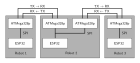
\includegraphics[width=\textwidth]{figures/communication_setup.pdf}
    \caption{The setup for our inter-module communication prototype. Physical
    realization is shown in figure \ref{fig:comm_setup_p}.}
    \label{fig:comm_setup}
\end{figure}

\begin{figure}[!t]
    \centering
    \includegraphics[width=\textwidth]{figures/com_setup.jpg}
    \caption{Physical realization of the setup shown in figure \ref{fig:comm_setup}.}
    \label{fig:comm_setup_p}
\end{figure}

We tested our implementation in a simple setup shown at figure
\ref{fig:comm_setup}. We used three ESP32-DevkitCs simulating module
controllers, and for Arduino Nanos simulating the docks. We wired them as shown
in the figure. Then, we were able to successfully establish both, TCP and UDP,
connections. The codes for establishing the connections are a simple example
inspired by official demo codes. There are no modifications for our setup. The
example codes can be found in the project repository.

Replication of our results should be fairly straightforward as we ship all the
code as PlatformIO\footnote{\url{https://platformio.org/}} projects, therefore
no complicated toolchain setup is necessary; and also, the hardware we use is
commonly available. However, during testing of our firmware, we encountered a
bug in lwIP implementation preventing a TCP connection from being opened. The
bug has been already fixed in the lwIP upstream repository, however, at the time
of writing this thesis, the lwIP library shipped with ESP-IDF was not updated.
Therefore, to successfully run the TCP example, manual update of the library is
necessary.

\section{Universal Module}

So far, we have built several prototypes of the universal module; some of the
key iterations are shown in figure \ref{fig:um_evolution}. There were several
challenges during the design of the module; first, the module should be as rigid
as possible to be able to support large structures of RoFI systems (this is
challenging mainly due to the presence of the $\gamma$-axis), second, the
internal arrangement of components have to be compact to fit in the 10cm cube
grid and third, the module should be strong to lift at least two other robots.

\begin{figure}[!t]
    \centering
    \includegraphics[width=\textwidth]{figures/um_evolution.jpg}
    \caption{Evolution of the universal module. First paper prototype (left),
    first 3D printed version (middle), and the current state (right).}
    \label{fig:um_evolution}
\end{figure}

The last prototype (figures \ref{fig:um_photo_side} and \ref{fig:um_photo_top})
fulfills our goals -- it features rigid construction and we were able to fit
sufficiently strong servomotors (Heculex DRS-0101) inside the body while still
leaving a reasonable amount of space for the control electronics and an
accumulator. The electronics and accumulator are supposed to fit in the central
part of the robot; some small components can be also placed in the cavity below
and above motors for $\alpha$- and $\beta$-axes.

\begin{figure}[!t]
    \centering
    \includegraphics[width=\textwidth]{figures/um_side.jpg}
    \caption{Universal module -- side view.}
    \label{fig:um_photo_side}
\end{figure}

\begin{figure}[!t]
    \centering
    \includegraphics[width=\textwidth]{figures/um_top.jpg}
    \caption{Universal module -- top view.}
    \label{fig:um_photo_top}
\end{figure}

The prototype was 3D printed using the same settings as the docking mechanism.
The CAD models are available in the project repository. To produce all
components for a single module 65 meters of a filament are needed with the print
time of 20 hours (docks are excluded from this list). The additional components
needed for assembling the robots are: 3 motors DRS-0101, 1 ball bearing
$25\times32\times4$~mm, 4 ball bearings $15\times20\times4$~mm, 4
M$2\times18$~mm screws with countersunk head, 18 M$2\times12$~mm screws with
countersunk head, 42 M$2\times6$~mm screws with countersunk head and 4
M$2\times12$~mm screws with a regular head. Assembling the modules takes about 1
to 2 hours of work, most of the time taking manual thread tapping.

We designed the components not to only be easily 3D printable but also to be
reasonably manufacturable by other techniques -- specifically milling (the body)
or sheet metal bending (the shoes). Such techniques could not only produce
stronger components from stronger materials but also, speed up the
manufacturing process.

\chapter{Conclusion}\label{chap:conclusion}

We presented a brand new platform for metamorphic distributed robots -- the RoFI
platform. The RoFI platform consists of autonomous modules which can form a
firm mechanical connection between the modules and therefore, create larger,
more sophisticated structures -- RoFI systems.

As the foundational element of the platform, we designed a docking system,
called RoFI dock, which provides a way to autonomously connect two modules, form
a firm mechanical connection, establish communication lines and share power
between the modules. We showed that the RoFI dock can be manufactured by
commonly available means and that it provides a reasonably reliable and robust
connection. Also, we designed the dock such that it is a self-contained device
which can be easily integrated into various modules.

On top of the docking system, we defined a what a module of the platform is. We
built a formalism to describe the modules and also the whole RoFI systems
consisting of multiple modules. Together with this formalism we also established
a terminology concerning the systems and their reconfiguration, so the
algorithms for reconfiguration can rely on it.

We also proposed and demonstrated a novel approach for communication between the
modules by adapting standard TCP/IP networking with a custom physical layer. The
usage of TCP/IP allows for seamless integration with other networks and possibly
the Internet, leverages robustness of well-tested protocols and also allows for
easy adaptation of state of the art network research.

As an application of the overall platform definition, we designed and built the
\emph{universal module}, which should serve as a simple building block of RoFI
systems. To support the universal module, we designed \emph{RoFI Driver} -- a
collection of libraries and protocols covering the basic functionality of the
modules. The library includes implementation of dock driver, network interface
or remote firmware update through dock native communication channel. We also
proposed a library to simplify writing of massively asynchronous firmware for
microcontrollers.

\section{Future Work}

The RoFI platform is an ambitious project with goals beyond the scope of this
thesis. In this thesis we took bottom-up approach -- we started with the design
the modules and gradually working up to higher levels of abstraction. In the
near future, we would like to continue in the bottom-up approach and turn the
RoFI dock into self-contained device ready to embed in modules (this boils down
mainly to adding a control circuitry); next, we would like to equip the
universal module with control circuitry and accumulators.

Having the hardware setup described above opens the possibility to take the
up-down approach and focus on the algorithmic aspects of the metamorphic modular
robots -- mainly control and reconfiguration. We would like to implement some
already published algorithms and validate them using the hardware setup provided
by the RoFI platform. Then we would like to explore the possibility of
controlling the RoFI systems in a distributed manner as the nature of the
modules seems suitable for distributed control and could leverage the
computational potential of all the robots in the system.

In the long term goals it could be also interesting to explore topics related to
security (how to prevent inter-module communication sniffing and manipulation),
specification (how to encode abstract task like "bring me a ball" into a
formalism suitable for machine processing) or control synthesis (how to find out
the sequence of actions to fulfill given task).

With more applications of the platform, we would like to revisit the design
choices we made and iteratively improve the platform. This might concern e.g.,
the arrangement of the universal module, physical layer for the communication or
the choice of the microcontroller.


\chapter*{Bibliography}
\addcontentsline{toc}{chapter}{Bibliography}
\markboth{}{} % avoid headers from last chapter in bibliography
\printbibliography[heading=none]

\appendix
\chapter{RoFI Driver Interface}\label{chap:rofi_interface}

The interface of the RoFI driver can be obtained by calling
\cpp{auto interface = rofi::getInterface()}. The
function returns an implementation defined object fulfilling concept
\cpp{RoFI}. The \cpp{RoFI} concept is an object such that:
\begin{itemize}
    \item \cpp{interface.joints} is a container-like object which
    \cpp{value_type} fulfills concept \cpp{Joint}.
    \item \cpp{interface.docks} is a container-like object which
    \cpp{value_type} fulfills concept \cpp{Dock}.
    \item \cpp{interface.self} is an object fulfilling concept \cpp{Module}.
\end{itemize}

\noindent An object \cpp{joint} fulfills concept \cpp{Joint} if:
\begin{itemize}
    \item \cpp{joint} can be copied (\cpp{Joint} is only a facade).
    \item \cpp{float Joint::max() const} returns a maximal join position in
    radians.
    \item \cpp{float Joint::min() const} returns a minimal joint position
    in radians.
    \item \cpp{float Joint::maxSpeed() const} returns a maximal joint speed
    in radians per second.
    \item \cpp{float Joint::maxTorque() const} returns the
    torque capability of a joint in N$\cdot$m.
    \item \cpp{float Joint::getPosition() const} returns the joint position.
    \item \cpp{float Joint::getSpeed() const}
    \item \cpp{void Joint::setTorque( float torque )} sets the joint into the
    torque movement control mode.
    \item \cpp{void Joint::setSpeed( float speed )} sets the joint into the
    speed control mode (constant velocity is kept) with given speed.
    \item \cpp{Pub< float > Joint::setPosition( float position ) }
    sets the joint into position control mode (position is kept). After the
    position is reached, the position emitted and stream is closed.
    \item \cpp{Pub< float > Joint::onPosition( float position ) const} emits a
    message whenever joint is in the given position (tolerance is implementation
    defined). The stream never ends.
    \item \cpp{SubPub< T, float > Joint::positionReached( float position ) const }
    after receiving a value of type \cpp{T} emits a \cpp{position} when the
    position is reached.
    \item concurrent commands are sequentialized.
    \item if one command aborts the previous one, an error is emitted.
\end{itemize}

\noindent Object \cpp{dock} fulfills concept \cpp{Dock} if:
\begin{itemize}
    \item \cpp{dock} can be copied (\cpp{Dock} is only a facade).
    \item \cpp{Pub< State > Dock::state() const } returns the dock current
    state.
    \item \cpp{Pub< State > Dock::connect() } expands the dock. A value is
    emitted one the final position is reached.
    \item \cpp{Pub< Void > Dock::waitForConnection()} waits in the expanded
    position for the mating side. Emits a value when mating side connects, then
    the stream closes.
    \item \cpp{Pub< Void > Dock::waitForDisConnection()} Emits a value when the
    mating side disconnects, then the stream closes. If there is no mating side,
    emits immediately.
    \item \cpp{Pub< Void > Dock::onConnection()} Emits a value when mating side
    connects. Never closes.
    \item \cpp{Pub< Void > Dock::onDisconnection()} Emits a value when mating
    side connects. Never closes.
    \item \cpp{Pub< MutualOrientation > Dock::getMutualOrientation()} returns
    a mutual orientation of docks.
    \item \cpp{Pub< Void > Dockd::disconnect()} retracts the dock. Emits once
    the target position is reached.
    \item \cpp{Pub< Void > Dock::connect( Line line ) } connect the EXT or the
    INT line. Once connected, a value is emitted.
    \item \cpp{Pub< Void > Dock::disconnect( Line line ) } connect the EXT or
    the INT line. Once connected, a value is emitted.
    \item \cpp{Pub< float > Dock::current( Line line ) } returns the current in
    Ampers at a given line.
    \item \cpp{Pub< float > Dock::voltage( Line line ) } returns the voltage in
    Volts at a given line.
\end{itemize}
Note that the high level interface does not provide a way to send data to
neighbors. The user application should rely on TCP/IP instead.

An object \cpp{module} fulfills concept \cpp{Module} if:
\begin{itemize}
    \item \cpp{module} can be copied (\cpp{Module} is only a facade).
    \item \cpp{Guid Module::getId() const} returns module GUID.
    \item \cpp{std::string Module::getType() const} returns a human-readable
    module type name.
    \item \cpp{ShapeDescriptor Module::getShape() const } returns a shape
    descriptor.
\end{itemize}

\end{document}
